\documentclass[10pt,twoside]{article}
\usepackage{dnd}
\usepackage[utf8]{inputenc}
\usepackage{multicol}                 % Multicolumn pages
\usepackage[hidelinks]{hyperref}      % Clickable table of content links

% Page Settings
\raggedcolumns
\setlength{\parindent}{0em}
\setlength{\parskip}{0.5em}

% Image directory
\graphicspath{ {images/} }

% Table settings
\newcolumntype{b}{X}
\newcolumntype{s}{>{\hsize=.5\hsize}X}
\newenvironment{powertable}{\rowcolors{2}{bgtan}{commentgreen}\longtable} {\endlongtable}
\newenvironment{standardtable}{
    \par\vspace*{8pt}
    \noindent
    \fontfamily{lmss}\selectfont %Select font
    \rowcolors{1}{bgtan}{commentgreen} % Alternate colors
    \tabularx
}
{\vspace{8pt plus 1pt}\noindent\endtabularx}
% Table Environment
\newenvironment{redtable}{
    \par\vspace*{8pt}
    \noindent
    \fontfamily{lmss}\selectfont %Select font
    \rowcolors{1}{bgtan}{itemtablepink} % Alternate colors
    \tabularx
}
{\vspace{8pt plus 1pt}\noindent\endtabularx}


% Start document
\begin{document}

  \section*{Broken Stars: Players guide}

  \begin{multicols}{2}

  \addtocounter{section}{1}

  Welcome to the Black, adventurer! 
        
  The year is 3210 and, despite all of the set-backs, humanity has streched out across the stars. We first escaped our ancient Cradle (an affectionate space-name for Earth) using simple "propulsion thrusters", and we terraformed and colonised the entire star system in just a few centuries. During this time we probably also figured out how to do \textit{real} artificial intelligence, put computers inside our brains, make laser weapons, and all of the other cool technology we use in our everyday lives.
        
  But the game-changer came with the invention of the Trans-Dimensional Drive, or TDD for short. This special machine allowed us to bend the laws of Space-Time for Faster Than Light (FTL) travel using what the tech-heads call "trans-dimensional energy". The TDD allowed us simple apes to escape the gravity of Sol and \textit{really} explore the big ol' Black.

  Civilisation continued to expand with each new colony founded, alien species encountered, and star sector charted. We started to link everything together using gigantic Jump Portals that allowed ships without their own TDD engine to travel at FTL speeds. The Black slowly fell to our ever-expanding hunger.
  
  We became so reliant on TDD technology that eventually people began to experience side-effects. When you are exposed to trans-dimensional energy for long periods of time you begin to change. Some lucky individuals developed the ability to manipulate Space-Time itself, while others became malformed or simply driven mad. These people became known as psionics, psychics, paranorms, or jsingshen. Whole Research Centres were made to study and train psionics so that their abilities could be used to stretch out even further across the stars.

  And then it all came crashing down.
        
  We call it \textit{The Surge}. It was a large shockwave of energy that exploded from deep within the center of the galaxy, sweeping across and overloading everything that used trans-dimensional energy. In a matter of seconds we lost our Jump Portals, TDD engines and even psionics to the Surge.

  In the aftermath, some worlds began to starve without the trade network built on FTL travel. Others slid into barbarism as they fought over dwindling resources. Countless worlds began their struggle for survival due to their sudden isolation. And the remaining Psionics had to learn to safely harness their powers without the guidance of experienced mentors.

  But over the last few centuries we have begun to rebuild. We turn our eyes to the edges of the Black once again. Warlords and petty tyrants scheme to expand their stellar domain. Reclaimers plunder the ruins of worlds that did not survive. Trade routes have been revived through the use of the Intra-Dimensional Drive (IDD), a less performant but safer derivative of the TDD. And Psionics practice their skills away from the distrustful eyes of those who see the use of trans-dimensional energy as an imminent threat to civilisation.

  \textbf{Good luck out in the Black!}
  
  \vspace{\baselineskip}
  
  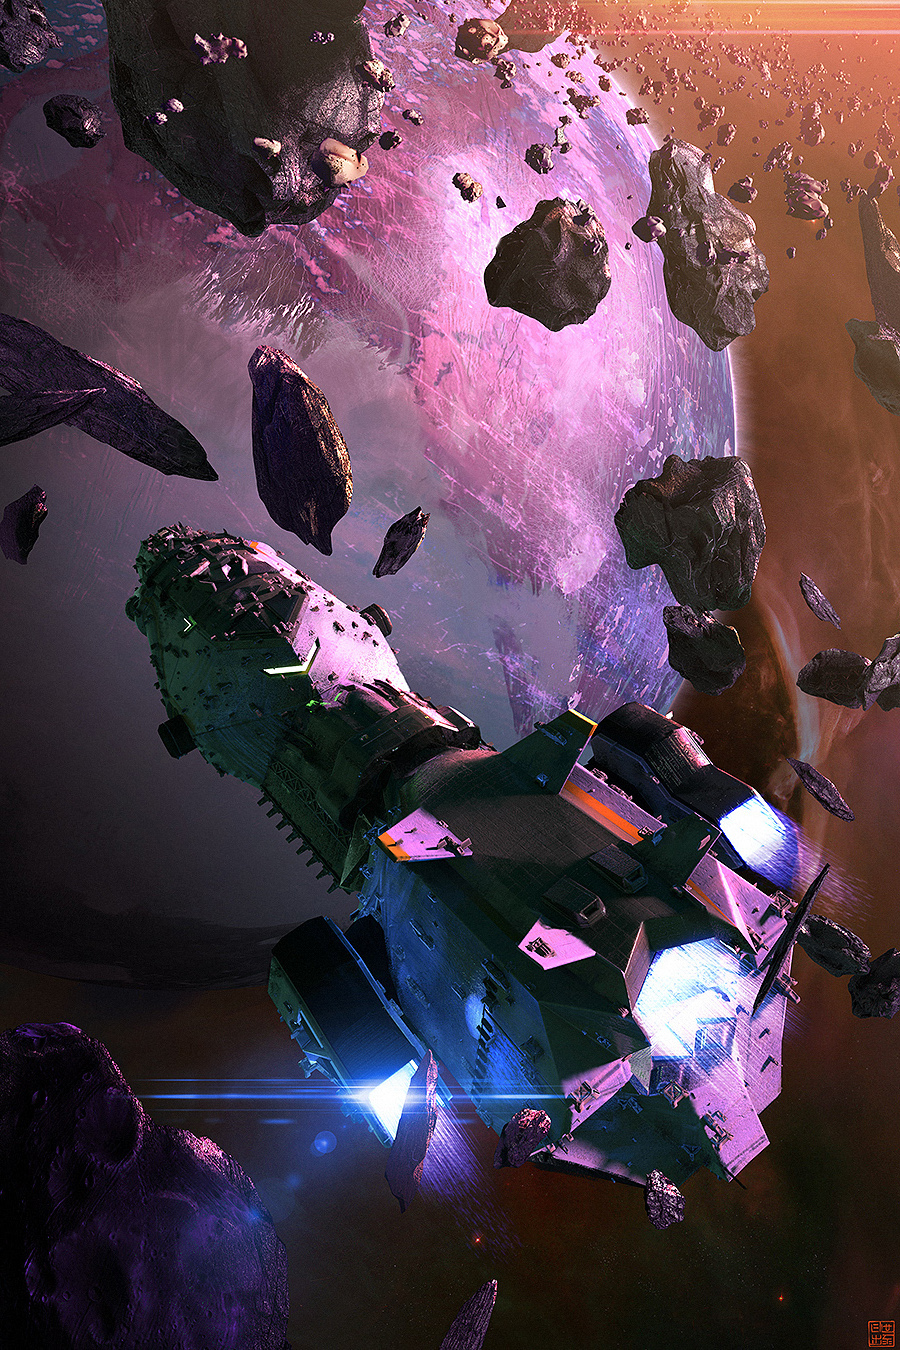
\includegraphics[width=\linewidth]{rebellion_of_stars___starship_blackbeard_by_hideyoshi-d8p607x}
  
  \newpage

  \tableofcontents
        
  \newpage

  % =================
  % The Rules
  % =================
  
  \section{The Rules}

  \subsection{Character Creation}
  
  \begin{enumerate}

    \item \textbf{Species}: The default species is human, although you can choose to play one of the many alien species.
    \begin{standardtable}{\linewidth}{sb}
      \textbf{Species} & \textbf{Description}\\
      Ay-Matak & Avian alien species that love to travel and experience life.\\
      Bots & Ranges from androids, robots, Ghosts, and everything in between.\\
      Ghantak & Insectiod alien species that are tradition and honour-bound.\\
      Ghoa & Violent and combative mammalian-reptilian hybrid alien species.\\
      Human & Stock-standard genetically unaltered human descended from Earth.\\
      Kaj & Intelligent grey-skinned humanoid alien species.\\
      Pluvma & Multi-limbed alien species that are drawn to the weird and quirky.\\
      Uplifted & Genetically-altered Earth animals that have been spliced with human DNA.\\
    \end{standardtable}

    \item \textbf{Attributes}: You start with a d4 in each attribute and have 5 points with which to raise them. Raising an attribute by one die type costs 1 point (but you cannot raise an attribute above a d12).
    
    \begin{standardtable}{\linewidth}{sb}
      \textbf{Attribute} & \textbf{Description}\\
      Strength & Raw physical power and general fitness.\\
      Agility & Nimbleness, quickness and dexterity.\\
      Smarts & Mental agility and your knowledge about the worlds that inhabit the Black.\\
      Spirit & Inner wisdom and willpower.\\
      Vigor & Endurance and a measure of how much pain and physical damage you can shake off.\\
    \end{standardtable}

    \item \textbf{Skills}: You have 15 points for skills. Each die type in a skill costs 1 point up to the linked attribute. Going over the linked attribute costs 2 points per level. A seperate list of skills is provided in it's own section.

    \item \textbf{Derived Traits}: Calculate your derived traits according using your attributes and skills.
    
    \begin{standardtable}{\linewidth}{sb}
      \textbf{Trait} & \textbf{Description}\\
      Charisma & Calculated as: \textbf{(Spirit / 2) - 4}. General likeability and manners, and is added to all persuasion and streetwise rolls.\\
      Pace & Calculated as: \textbf{(Strength / 2) + 2}. How many squares of movement you can take during your turn.\\
      Parry & Calculated as: \textbf{(Fighting / 2) + 2}. Target number for melee combat or against ranged weapons within melee range.\\
      Toughness & Calculated as: \textbf{(Vigor / 2) + 2}. Add armour on top of toughness.\\
    \end{standardtable}

    \item \textbf{Hindrances}: You can choose to gain additional character creation points by taking up to \textbf{one} Major Hindrace (2 points) and up to \textbf{two} Minor Hindrances (1 point each).
    
    \begin{itemize}
        \item For 2 points you can gain another attribute point or choose an \textbf{Edge}. 
        \item For 1 point you can gain another skill point or increase starting funds by 100%.
    \end{itemize}
            
    \item \textbf{Edges}: Edges are what sets your character apart from everyone else. There are 3 main paths to choose from:
    
    \begin{itemize}
        \item \textbf{Standard}: Just use the normal Edge list. 
        \item \textbf{Psionic}: Take the \textit{Psionic Background} edge and manipulate Space-Time.
        \item \textbf{Cyberware}: Take the \textit{Cyberware Install} edge and meld flesh with machine.
    \end{itemize}

    \item \textbf{Gear}: All characters start with 750 Credits to buy their equipment with.

    \item \textbf{Background Detail}: Fill in any other details of your character's background.

  \end{enumerate}
        
  \columnbreak
  
  \subsection{Advancement}
  
  Experience points are gained by completing a game session (of around 4-6 hours of gaming). Each game session is worth around 1-3 points. Unlike other role-playing games, instead of levels your character has a "\textbf{Rank}". Characters that have earned a higher rank are able to access the better Edges.
  
  \begin{standardtable}{\linewidth}{sb}
      \textbf{XP} & \textbf{Rank}\\
      0-19 & Novice\\
      20-39 & Seasoned\\
      40-59 & Veteran\\
      60-79 & Heroic\\
      80+ & Legendary\\
    \end{standardtable}
  
  Every 5 points accumulated grants the character an Advance (or 4 Advances per Rank). One Advance allows you to do the following:
  
  \begin{itemize}
    \item Gain a new Edge
    \item Increase one skill that is equal to or greater than its linked attribute
    \item Increase two skills that are lower than its linked attribute
    \item Buy a new skill at d4
    \item Increase one attribute (only choose this once per Rank, and no Trait can be raised above a d12)
  \end{itemize}
  
  \subsection{Game Concepts}
  
  \begin{itemize}
    \item \textbf{Aces:} If you roll the highest number on any die, player rolls that die again and adds that to total
    \item \textbf{Basic test:} Roll die over Target Number
    \item \textbf{Bennies:} Players get 3 Bennies at start of the game. They’re for re-rolls and other things
    \item \textbf{Bleeding Out:} Make a Vigor roll every round until they are Stabilized. This happens before cards are dealt.
      \begin{itemize}
        \item \textbf{Success:} Roll again every round until Stabilized
        \item \textbf{Raise:} Stabilized. No more rolls
        \item \textbf{Fail:} Character dies
        \item If other characters make Healing rolls, character stabilizes – no more rolls
      \end{itemize}
    \item \textbf{Incapacitated:} After suffering 3 wounds make a Vigor roll:
      \begin{itemize}
        \item 1 or Less = Character dies
        \item Fail = Roll on Injury Table and effect is permanent. You are Bleeding Out
        \item Success = Roll on Injury Table. Injury gone when healed
        \item Raise = Roll on Injury Table. Injury gone in 24 hours
      \end{itemize}
    \item \textbf{Initiative:} Players get one card per turn and act according to the deck order, going from the Ace to Deuce (in case of ties the suit order is Spade, Heart, Diamond, Club). If the player gets a Joker they can act when they wants, and the Joker gives the PC +2 on all Tests and +2 to Damage
    \item \textbf{Opposed Rolls:} Defending player rolls. Their roll becomes other player’s Target Number
    \item \textbf{Raise:} Every 4 points over Target Number is a Raise and can give additional benefits
    \item \textbf{Shaken:} Characters are Shaken when they first take damage. On their next turn, make an immediate Spirit roll (\textit{May use Bennies to remove Shaken without a roll}) 
      \begin{itemize}
        \item \textbf{Success} = Not Shaken but may only do Free Actions
        \item \textbf{Raise} = Not Shaken and may act normally
        \item \textbf{Failure} = Still Shaken, may only do Free Actions.
      \end{itemize}
    \item \textbf{Soak Roll:} Spend a Benny on a Soak Roll (Vigor check) to regain 1 Wound. Raises take away +1 Wound per Raise. If all the wounds are Soaked it removes any Shaken condition
    \item \textbf{Unskilled:} If you are unskilled then your roll is a d4 with a –2 penalty
    \item \textbf{Wild Die:} A d6 rolled along with normal die. Player chooses highest result (but Snakeyes is a critical fail). Can Ace and Raise on the Wild Die
    \item \textbf{Wounded:} All characters have 3 Wounds until they are Incapacitated (Extras have 1 Wound). Damage and Raises when Shaken makes 1 Wound each. Each wound is –1 to Pace and all Trait Tests. (\textit{May use Bennies to make a Soak Roll})
  \end{itemize}
  
  \columnbreak

  % =================
  % Species
  % =================

  \section{Species}

  \subsection{Ay-Matak}
  
  \begin{redtable}{\linewidth}{sb}
    \textbf{Height} & 135-170cm\\
    \textbf{Weight} & 45-65kg\\
    \textbf{Gender Ratio} & 40\% Male / 60\% Female\\
    \textbf{Reproduction} & Oviparity (Eggs)\\
    \textbf{Diet} & Omnivore\\
    \textbf{Homeworld} & Matak (Lost)\\
  \end{redtable}

  The Ay-Matak (\textit{plural: Ay-Matakian}) are an alien species that have evolved from the birds native to their homeworld of Matak. They typically shorter and lighter than humans, have two pairs of wings, are bi-pedal, and have two arms with opposable thumbs on each of their hands. The beak is solid and sharp along the sides, with the tip made out of softer material that is flexible enough to produce a variety of sounds. The plumage of a male Ay-Matak is always more colourful than the female (who are limited to whites, greys and blacks).

  Their homeworld of Matak has been lost, leaving many Ay-Matak have been stranded across the black. Legend has it that Matak was reknowned for its tall trees that almost touched the edges of the atmosphere. It also had a rich ecosystem that meant the Ay-Matak enjoyed an overabundance of food and had little need to compete for limited resources. Because of this the Ay-Matak were able to fully indulge in the pleasures of life. The Ay-Matak place a high social value on the arts (especially those that use an abundance of colour or visual stimuli), travel, and new ideas.

  Planets with a majority of Ay-Matak are usually formed under an Oligarchic government. The members of the government are generally influential elders who have contributed greatly to the culture of the planet, or have travelled far and wide in search of new ideas.

  Ay-Matakian characters have the following traits:
  \begin{standardtable}{\linewidth}{sb}
    \textbf{Flight} & Can fly at their basic Pace and even "run" while flying. It cost 2 squares of Pace to gain 1 square of height.\\
    \textbf{Hollow-boned} & -1 toughness.\\
    \textbf{Free Edge} & Start with one free Novice Edge of their choice, regardless of requirements (except those that require other Edges).\\
  \end{standardtable}
  
  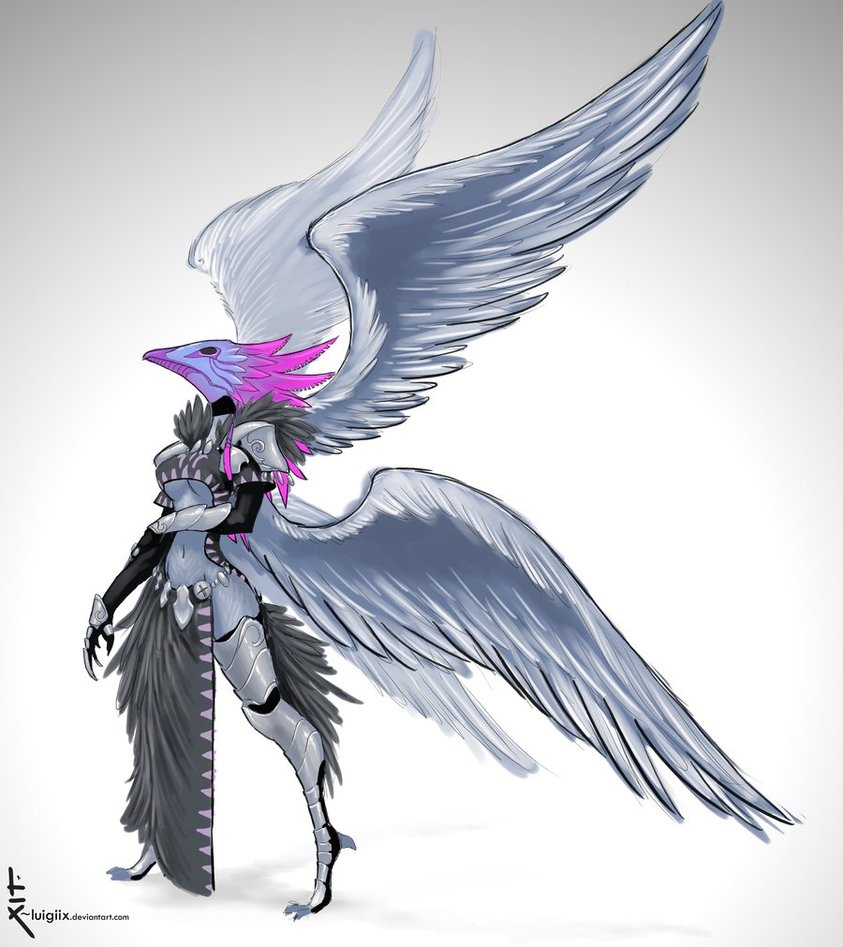
\includegraphics[width=\linewidth]{bird_race_f_concept_by_luigiix-d52w3as}
  
  \textbf{Male Names}: Andomion, Antakon, Artenaeon, Demoleo, Dralop, Entardion, Eraton, Eratro, Heliodo, Ikotu, Kalipon, Koron, Lokinu, Melaleimon, Myrodon, Panolio, Taramio, Teladon, Tridru, Tyrorion
  
  \textbf{Female Names}: Agara, Alanie, Aldorria, Anakia, Atria, Bellaleta, Belliana, Hallia, Iripira, Karellia, Katia, Kynie, Laleta, Nerian, Nolanta, Obemona, Peneleta, Talitian, Tiakia, Utriema
  
  \textbf{Secondary Names}: Ay-Matak do not take family names, but instead earn cultural "\textit{titles}" for their last well-known greatest achievement. For example, \textit{Andomion, painter of 'Matak Lost'}. Those without a great achievement usually go by their occupation, birthplace, spacecraft name, or include the name of their mother ("\textit{hatchling of Anakia}"). Needless to say that many an Ay-Matak have caused headaches for human bureacrats.
  
  \columnbreak

  \subsection{Bot/Shell}
  
  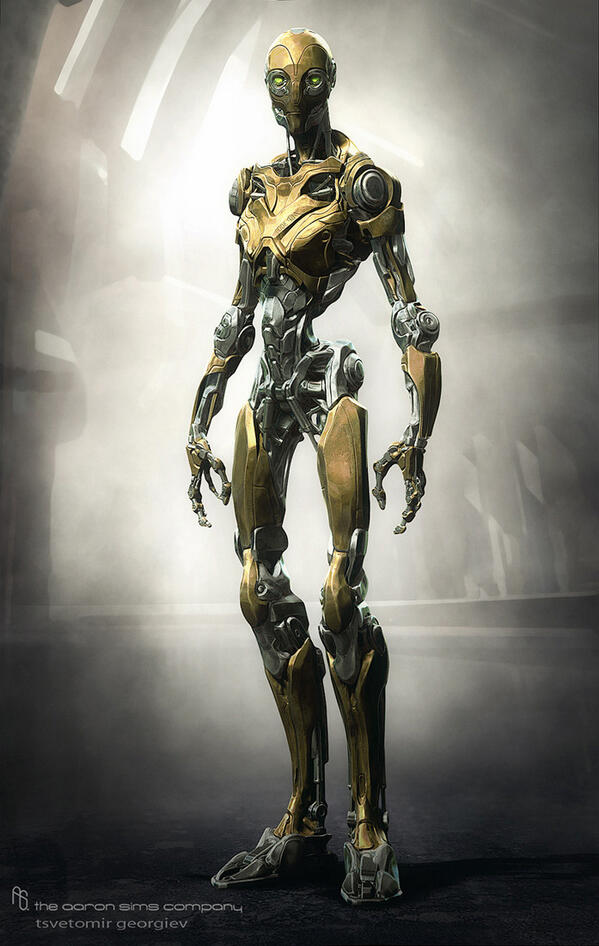
\includegraphics[width=\linewidth]{BEzZuPdCEAAgcr8}

  A common sight on any technologically-advanced society is the large number of Bots and machines performing menial yet necessary labour. Most of these machines are limited to a singular purpose and have a "weak AI". But technology has advanced far enough that some robots can be programmed to display human-like cognitive abilities. These Bots are considered to have "strong AI", and are used for highly specialised and complex work.
  
  On the other end of the spectrum are individuals who have made the transition from organic to mechanical. These individuals, known as Ghosts, have chosen to digitise their conciousness and memory and upload themselves into artificial bodies known as Shells. Many in society believe that these digitised conciousnesses have lost their basic "humanity", and are indistinguishable from normal AI. 
        
  Bot and Shell characters have the following traits:
  \begin{standardtable}{\linewidth}{sb}
    \textbf{Construct} & Add +2 to recover from being Shaken, do not suffer wound modifiers, and are immune to poison and disease. They cannot Heal naturally, and require the Repair skill to remove wounds (use like the Healing skill).\\
    \textbf{Artificial} & Organic races often mistrust and misunderstand Bots and Shells. -2 to Charisma when dealing with races other than their own.\\
    \textbf{Programming} & Start with one free d6 in one skill, representing their original programmed role.\\
    \textbf{Recharge} & If you cannot access a power source at least once a day, suffer one point of Fatigue each day until incapacitated. The day after that, you go "off-line" and must be revivied with a Repair roll and a four-hour charge. This replaces the need for food and water, unless food and water is selected as the power source.\\
  \end{standardtable}
  
  \begin{commentbox}{Playing as a Bot}
  \textit{Swapping Bodies}: Since you are a digital conciousness (Ghost or AGI), you may decide to change your form-factor for a chassis more suited to the task at hand (after acquiring it, of course). You will experience disorientation as you get used to your new chassis. The settling period usually occurs over a few days (at the GM's discretion), after which you will be totally fluent in the capabilities of your new body. Once you have changed bodies, replace your original "\textit{Programming}" ability with another one more suited to your new chassis. You may also have a new power source.
  
  \textit{Hacking}: Hacking and reprogramming a Bot is a very complex task. It will generally require the Hacker to access a physical IO port (most computer and electronic systems guard against remote entry), which is best accessed if the Bot is incapacitated. Then the Hacker needs to open the IO port (Hacker's Repair vs Bot's Toughness), and then break the software Firewalls (Hacker's Security opposed by the Bot's Spirit).
  
  \textit{Artificial}: Most organic beings have an inherent distrust of AGI and see the machines as a threat. Machines are depicted (rightly or wrongly) as unfeeling, ruthlessly efficient, and simply cannot "get it". Characters will generally prefer to deal with an organic "master", and are wary of any machine that claims it is operating independently.
  \end{commentbox}
  
  \columnbreak

  \subsection{Ghantak}
  
  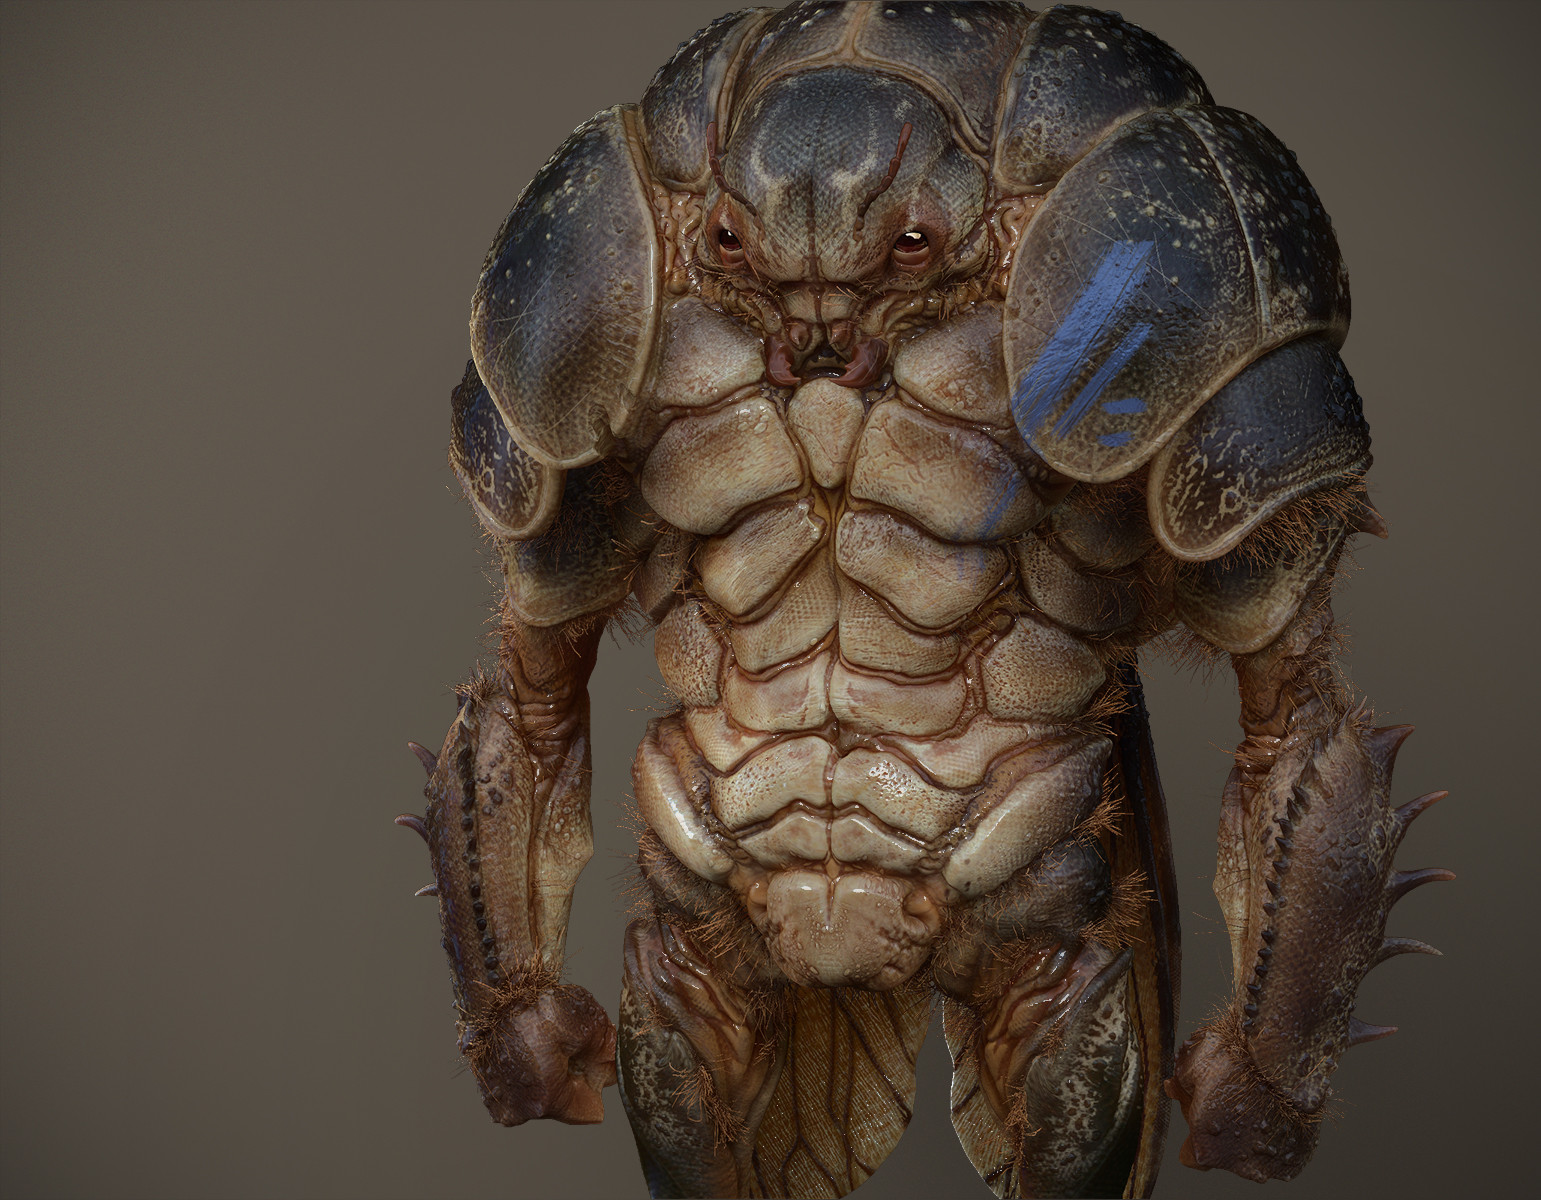
\includegraphics[width=\linewidth]{bruno-camara-beetle-brunocamara}
  
  \begin{redtable}{\linewidth}{sb}
    \textbf{Height} & 135-170cm\\
    \textbf{Weight} & 55-90kg\\
    \textbf{Gender Ratio} & 90\% Genderless / 9\% Male / 1\% Female\\
    \textbf{Reproduction} & Ovuliparity (External egg fetilisation egg)\\
    \textbf{Diet} & Herbivore\\
    \textbf{Homeworld} & Ghan\\
  \end{redtable}
        
  The Ghantak (\textit{plural: Ghantakian}) are an alien species evolved from the beetle-like insects native to their homeworld of Ghan. They are shorter than humans but weigh about the same, have an armoured carapace that covers their whole body, and their head is between the shoulders where the human chest would be. The odd placement for a Ghantakian head means that they must turn their whole body to look around.
  
  Although each individual has their own free will, the Ghantak as a species have an innate tendancy to organise themselves into highly-structured hierachies. Most Ghantak highly value honour and tradition, with personal sacrifice to uphold Ghantakian values earning an individual glory and esteem. The race generally favours traditional solutions to problems, and individuals are uncomfortable when forced to exercise their own judgement.
  
  While there used to be multiple independant hierarchies (each with their own Queen), the entire modern Ghantakian society is now ruled by a singular Empress. The Empress is chosen from the Queens of the remaining hierarchies and she rules until her death.
         
  Ghantakian characters have the following traits:
  \begin{standardtable}{\linewidth}{sb}
    \textbf{Carapace} & You have an armoured carapace that protects you from harm. +2 Armour.\\
    \textbf{Reputable} & Your species is seen as dependable, loyal and predictable. +2 charisma when dealing with characters who have heard of the Ghantak before.\\
    \textbf{Restricted senses} & Your unsual head restricts your field of vision and hearing. -2 to Notice rolls requiring vision and hearing\\
  \end{standardtable}
  
  \textbf{Ghantakian Names}: Akiesuh, Bazoh, Bolbih, Choxu, Etix, Farqae, Gaknu, Graux, Greex, Havzal, Leksur, Mamobah, Mezuat, Semunu, Sydesih, Thonox, Vexoh, Zimla, Zouh, Ziuzoch
  
  \textbf{Secondary Names}: Ghantak do not take secondary names. Ghantakian first names are generally unique enough for a specific region. If pressed, the Ghantak will choose the next available incremental number for the region and their name. 
  
  \textbf{Males and Females}: Females are especially reverred in Ghantakian culture, and are fanatically protected by all Ghantakians. They are rarely seen by non-Ghantakians, but can be differentiated by their large birthing pouch located just above their rectum. Males are also important to Ghantakian society, and usually are kept close to females to help breed the new generation. Males are allowed to travel the Black, and are almost indistinguishable from the genderless Ghantak (their genitalia is usually sheathed and protected by their carapace).
    
  \columnbreak

  \subsection{Ghoa}
      
  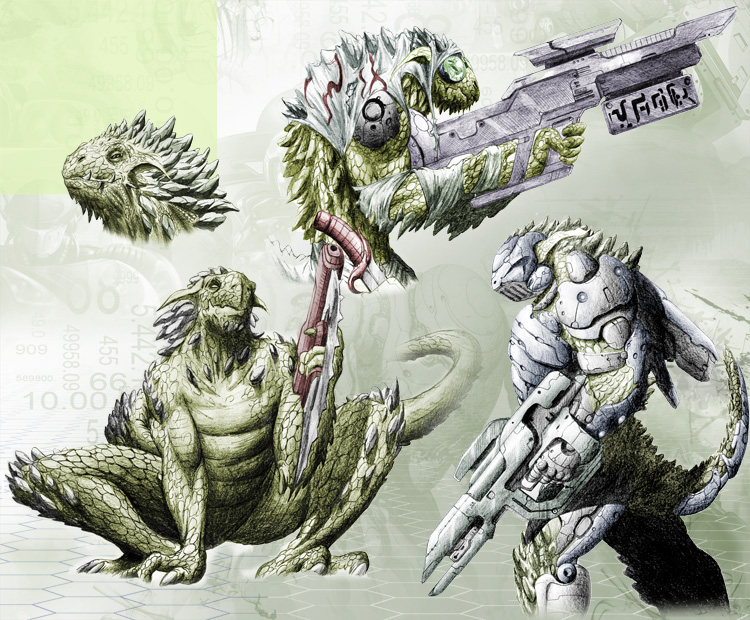
\includegraphics[width=\linewidth]{alien_reptile_concept_by_xjager513-d3ba4g7.jpg}
  
  \begin{redtable}{\linewidth}{sb}
    \textbf{Height} & 170-220cm\\
    \textbf{Weight} & 70-130kg\\
    \textbf{Gender Ratio} & 100\% Hermaphrodite\\
    \textbf{Reproduction} & Viviparity (Live birth)\\
    \textbf{Diet} & Omnivore (meat preference)\\
    \textbf{Homeworld} & (\textit{Unknown})\\
  \end{redtable}
        
  The Ghoa (\textit{plural: Ghoan}) are an alien species evolved from an unusual mammal-reptile hybrid native to their homeworld. Their homeworld has been lost to time as the Ghoa place little value on sentimental ties and recorded histories. They are larger and heavier than humans, with sharp ridged scales covering their back. They also have sharp claws and teeth, and have been known to use their tail as a weapon.
  
  The Ghoa are typically tribal, putting their tribe ahead of all other social groups (including the species as a whole). Their chief mode of expression is anger, and the Ghoa are prone to acts of wanton violence. Disputes are traditionally resolved through force, but rarely to the death. Some Ghoa actively embrace the honour and glory of death in battle, and actively seek out combat as mercenaries and pirates.
  
  All Ghoa are hermaphrodites, meaning they have both male and female genitals. Pregnancy is an undesirable period for any Ghoa (as it makes you weaker and more vulnerable during combat), so "females" are usually the Ghoa who are incapable of fighting and have been forced to be subservient to other Ghoa (usually the whole tribe). "Females", or "Breeders", are constantly pregnant in order to produce many warriors for the tribe.
    
  Ghoan characters have the following traits:
  \begin{standardtable}{\linewidth}{sb}
    \textbf{Bigger \& Heavier} & Ghoa are larger than other races. Start with a d6 in Strength instead of a d4.\\
    \textbf{Bloodthirsty} & Ghoa are cruel to their foes, rarely take prisoners, and feel little compunction about punishing captured enemies. This causes a -4 Charisma penalty when dealing with "civilised" worlds that know of the Ghoa.\\
    \textbf{Natural Weapons} & The Ghoa use their tails, claws and teeth as weapons, dealing Str+d6 damage.\\
    \textbf{Tribal Warriors} & Their willingness to use violence to solve all problems mean that the Ghoa start with a d6 instead of a d4 in the Fighting skill.\\
  \end{standardtable}
  
  \textbf{Ghoan Names}: Bonmok, Chardo, Drothax, Druthak, Dunmom, Garuga, Grintaz, Krudrar, Lakuq, Lugrub, Mugarod, Okrih, Pok, Rok, Roslarb, Sabub, Shak, Shopurd, Trougha, Zugorim
  
  \textbf{Secondary Names}: Ghoa use their tribe as a secondary name. Tribal names are usually descriptive, grandiose, or violent. Tribes are extremely fluid, as new ones are created all the time and do not need to be limited to the Ghoa only (some Ghoa see their teammates as part of their "tribe" and will take on the spacecraft name). 
    
  \columnbreak
      
  \subsection{Kaj}
  
  
\includegraphics[width=\linewidth]{7e9dc5cf139ae3df9568cfd9921ba9b5}
  
  \begin{redtable}{\linewidth}{sb}
    \textbf{Height} & 150cm\\
    \textbf{Weight} & 55kg\\
    \textbf{Gender Ratio} & 100\% Clones\\
    \textbf{Reproduction} & Cloning\\
    \textbf{Diet} & Omnivore\\
    \textbf{Homeworld} & -\\
  \end{redtable}
  
  The Kaj (\textit{plural: Kaj}) are a highly intelligent species that have long ago decided to abandon the natural world and fully embrac artificial environments. The Kaj even went so far as to reject sexual reproduction and replace it with genetic engineering and cloning. While cloning has allowed the Kaj to artifically raise the intellectual quotient of their species, it has also left them susceptible to genetic diseases and viruses. This weakness to disease means that most Kaj keep a wary distance from outsiders, and zealously practice the highest hygiene standards and procedures.
  
  They have also rejected their natural home planet, erasing the co-ordinates so that no Kaj could ever return. The Kaj generally choose to live in artificial spaces such as spacecrafts, space stations, and bubble colonies. To other species it seems that the Kaj have a driving desire to control their environment, but to most Kaj it is simply that they know better than the random processes that create the natural world.
  
  Their is a schism of thought within Kaj society about whether or not the species as a whole should embrace the artifical completely and digitise their consciousness. Some see Digitisation as the logical continuation of the Kaj improving upon the natural, while many fear that Digitisation is a false path and would lead to the eradication of the Kaj as a species (and culture) from the galaxy. There is a whole spectrum of opinion regarding Digitisation, and this opinion usually manifests itself through how much cyberware the Kaj has. A minority of Kaj even reject the cultural acceptance of the artifical, and aim to help the Kaj rediscover the natural world.
  
  Kaj characters have the following traits:
  \begin{standardtable}{\linewidth}{sb}
    \textbf{Genetically enhanced} & Kaj start with a d6 in Smarts instead of a d4.\\
  \end{standardtable}
  
  \textbf{Ghoan Names}: Abupikal, Brohekano, Debimaum, Fawaroum, Frukasoiro, Gatuxund, Hanepim, Ibaxi, Nothano, Osoluga, Qitandok, Romazirash, Rumduvish, Schapruga, Strikzan, Tirwein, Xintegi, Zefinag, Zosdash, Zulaum
  
  \textbf{Secondary Names}: Kaj usually use the location of their cloning facility as a secondary name. Each cloning facility keeps extensive records on names to ensure that they are completely unique to the individual, such that no two Kaj from the same facility will ever have the same name across the working life of the facility. 
  
  \columnbreak
  
  \subsection{Pluvma}
  
  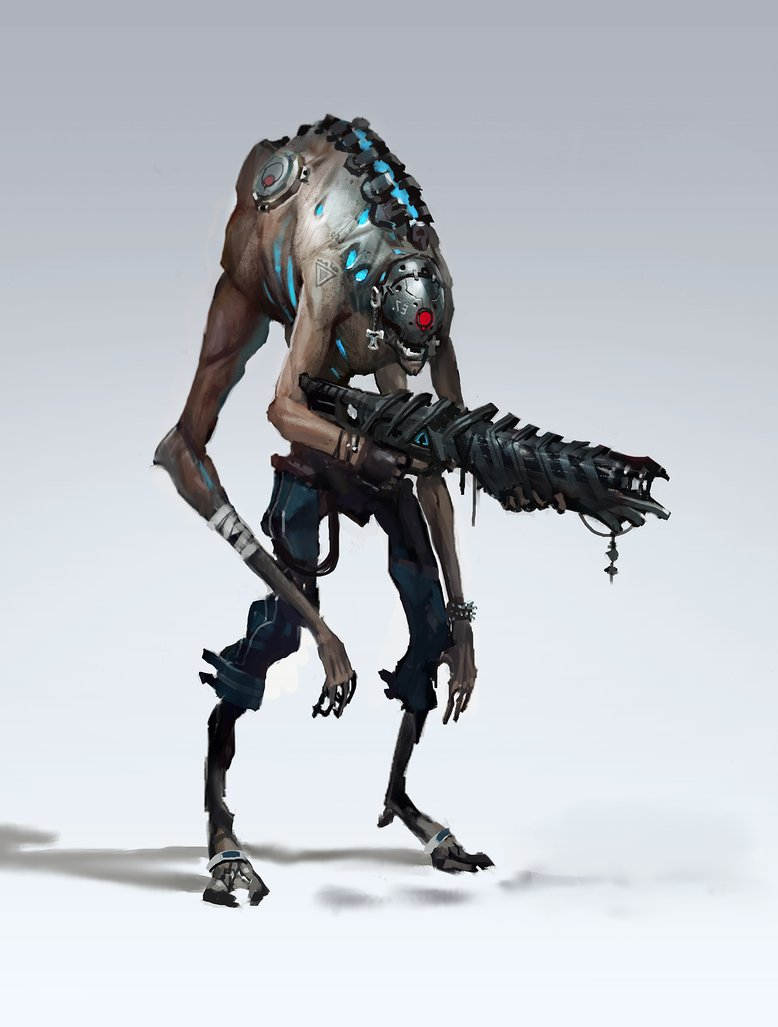
\includegraphics[width=\linewidth]{soldier_by_zoonoid-d4qf4cg}
  
  \columnbreak
  
  \subsection{Human}
  
  
\includegraphics[width=\linewidth]{TCP-Pirate-2}
  
  \begin{redtable}{\linewidth}{sb}
    \textbf{Height} & 150-200cm\\
    \textbf{Weight} & 55-115kg\\
    \textbf{Gender Ratio} & 50\% Male / 50\% Female\\
    \textbf{Reproduction} & Viviparity (Live birth)\\
    \textbf{Diet} & Omnivore\\
    \textbf{Homeworld} & Earth\\
  \end{redtable}
  
  There are various types of humans seen in the Black. Some are proud of their genetic lineage tracing all the way back to Sol. Others are escaped clones that were destined to be uploaded with someone else's cortical stack. Even more are genetically altered humans, designed for the specific conditions of their colony during the Pre-Surge days. All of these different varities, no matter how weird or alien, are still considered human.
  
  Humans have the following traits:
  \begin{standardtable}{\linewidth}{sb}
    \textbf{Free Edge} & Start with one free Novice Edge of their choice, regardless of requirements (except those that require other Edges).\\
  \end{standardtable}
    
  \columnbreak

  \subsection{Uplifted}
      
  Uplifted is the general name given to the genetically-engineered animals that have been given basic sentience and humanoid features. The original reason behind this science experiment has long been lost, but many speculate that the Uplifted were supposed to perform the menial labour on planets that cannot support a Bot network. Regardless, the Uplifted are still treated as an inferior species because of their artificial evolution.
      
  All Uplifted have the following traits:
  \begin{standardtable}{\linewidth}{sb}
    \textbf{Inferior} & Many see the Uplifted as inferior to other species that have evolved naturally. -2 Charisma when other characters deal with the Uplifted.\\
    \textbf{Primal Strength} & You start with a d6 instead of a d4 in Strength\\
    \textbf{Primal Weapons} & You still have the claws, teeth, horns or other leftovers from your primitive animal state. These natural weapons do Str+d6 damage.\\
    \textbf{Primitive Intellect} & You must spend 2 points per step to raise your Smarts during character creation\\
  \end{standardtable}
  
  In addition, Uplifted have additional abilities due to their animal ancestry. Choose one of the following:
  
  \begin{standardtable}{\linewidth}{sb}
    \textbf{Bear} & Descended from Bears, you are as big (if not bigger) than most Ghoa. Usually police and military support. +1 Size, and +1 Toughness\\
    \textbf{Bovine} & Descended from Cows, Bulls, and Buffalo. Usually farmers and labourers. You start with a d6 in Vigor instead of a d4\\
    \textbf{Canine} & Descended from Wolves and Dogs. Usually police and military grunts. +2 to Notice when using smell or hearing\\
    \textbf{Feline} & Descended from Lions, Tigers and Panthers. Usually solitary military agents. Low-light vision (ignore penalities for dim and dark lighting), and +2 to Athletics climbing checks\\
    \textbf{Rodent} & Descended from Rats, Racoons, and Rabbits. Usually couriers (and, some speculate, spies). +4 Pace\\
  \end{standardtable}
  
  \columnbreak
  
  Uplifted physically range wildly across the spectrum from humanoid to their base animal form, but all Uplifted have at least a humanoid-style torso that have two arms with opposable thumbs (for manipulating objects). Faces may or may not have a prominent snout, and some uplifted do not have a tail. Almost all Uplifted have the fur coat of their base animal base form, but some choose to partially shave or style it to better fit in humanoid society.
  
  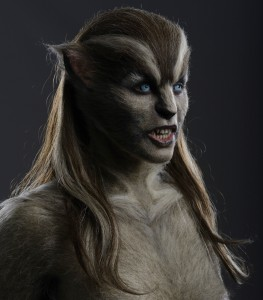
\includegraphics[width=\linewidth]{wolves-movie-still-1-263x300}
  
  Due to their severe genetic alteration and base animal genetics, Uplifted cannot breed with humans or with their animal precedessors. This does not deter kinky humanoids, and many unsavoury places in the Black offer "special" Uplifted services. However the heart wants what it wants, and Uplifted-Human couples are a rare sight in the Black. These couples generally seek out geneticists who are able to splice their DNA into viable offspring.
  
  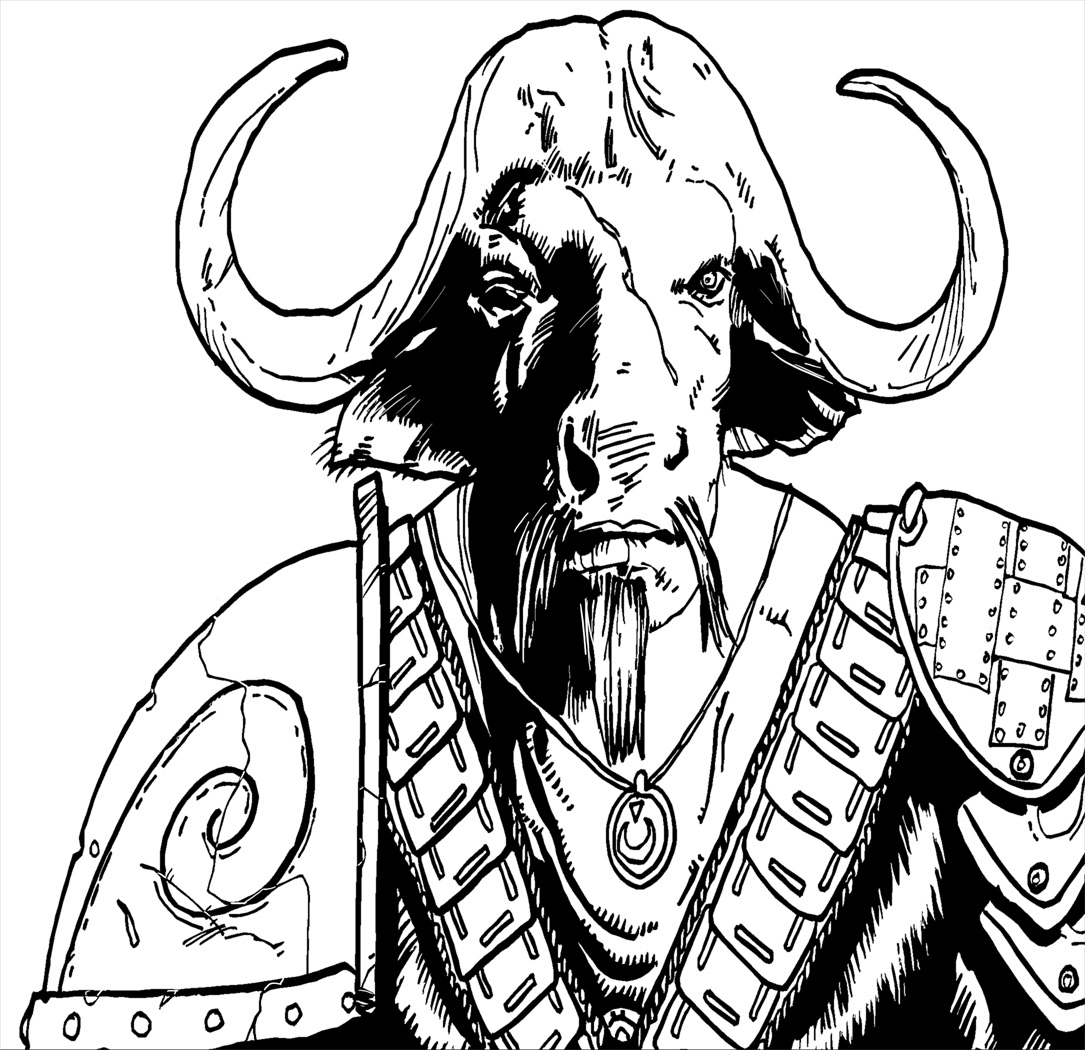
\includegraphics[width=\linewidth]{TCP-Armored-6}
  
  
\includegraphics[width=\linewidth]{charlesliu_bearman.jpg}
  
  \end{multicols}
  
  \newpage

  % =================
  % Skills
  % =================

  \section{Skills}
  
  \begin{powertable}{ p{.25\textwidth} p{.65\textwidth} }
    \textbf{Skill} & \textbf{Examples}\\
    Astrogation & Navigating safe FTL travel through the Black\\
    Astronautics & Designing and building a spacecraft (only need Repair to fix spacecraft)\\
    Athletics & Swimming, climbing, running, pushing, pulling, and weight-lifting\\
    Battle & Military strategy and tactics. Useful for running large combat operations\\
    Computers & Computers, Cyberware, Electrical, Electronics, Robotics and other computer theory\\
    Driving & Control any type of ground or water vehicle (including riding animals)\\
    Fighting & Covers all hand-to-hand (melee) attacks and thrown weapons (from grenades to spears)\\
    Healing & First Aid andtreating existing injuries (Success and raise eliminates 1 wound). Must subtract patients wounds in addition to own wounds when making a Healing roll\\
    Insight & Understand the motives or thoughts of someone, and scrutinizing people to see if they are lying\\
    Intimidation & Frightening enemies and making threats\\
    Knowledge (-) & Other area of expertise outside of "common knowledge" (which includes local history, etiquette, and operating common machinery and technology for their native tech-level\\
    Language (-) & One Non-native language. (\textit{d4 = common phrases, d6 = halting conversation, d8 = fluent, d10 = mimic dialects, d12 = recite important literary works})\\
    Life Sciences & Biology, Botany, Ecology, Exobiology, Genetics, Xenobiology, and Zoology\\
    Medicine & Latest medical theories on surgery, disease diagnosis, and epidemic containment\\
    Notice & General alertness, searching for items, and detecting ambushes\\
    Operations & Operate sensors, shields, communications and other spacecraft systems\\
    Persuasion & Convincing others. Five personality states are Hostile, Uncooperative, Neutral, Friendly and Helpful\\
    Piloting & Control any type of air or space craft\\
    Planetary Sciences & Geology, Hydrology, and Meteorology\\
    Psionics & Required for psionic characters to use their powers. For non-psionic characters, this skill represents their understanding of how psionics work\\
    Repair & Fix gadgets, vehicles, weapons and other machines. Apply -2 penalty if you do no have the required tools\\
    Science & Chemistry, Mathematics, Mechanics, and Physics\\
    Security  & Hacking, disarming traps, bypassing alarms, cyptography, and opening locks. Use this skill to protect against intruders\\
    Shooting & Covers all ranged attacks. Short range = 4, Medium range = 6 and Long range = 8\\
    Social Sciences & Archeology, Economics, Law, and Political Science\\
    Stealth & Hide and move quietly, as well as palm objects and pick pockets\\
    Streetwise & Gather information from people (to gather information from media use investigation). Includes tracking people in urban environments\\
    Survival & Find food, water and shelter in hostile environments. Includes tracking people in natural environments\\
    Taunt & Test of will attack against an opponent\\
  \end{powertable}

  \newpage
  
  % =================
  % Hindrances
  % =================

  \section{Hindrances}
  
  \textbf{Note:} Because Cyberware replacements are available, some Hindrances (like \textit{Blind}, \textit{Hard of Hearing}, \textit{One Arm}, \textit{One Eye}, and \textit{One Leg}) should not be available during character creation unless you take \textit{Cyberware Intolerance} to make the disability permanent. These disabilities remain on this list in case your character suffers an unfortunate injury.
  
  \begin{powertable}{ p{.20\textwidth} p{.10\textwidth} p{.60\textwidth} }
    \textbf{Name} & \textbf{Type} & \textbf{Description}\\
    All Thumbs & Minor & -2 penalty to Repair, and a natural 1 on the skill die (regardless of wild die) causes a malfunction\\
    Anemic & Minor & Prone to sickness, disease, and fatigue. -2 from all Fatigue checks (including those to resist poison and disease)\\
    Arrogant & Major & Must humiliate an opponent (i.e. disarm then hand weapon back), and will always challenge the "leader"\\
    Bad Eyes & Minor & -2 to attack or notice more than 5 squares away (unless wearing glasses)\\
    Bad Luck & Major & One less Benny per session\\
    Big Mouth & Minor & Unable to keep a secret, and blabs at the worst time\\
    Blind & Major & -6 to all tasks that require vision, and -2 to social tasks (as you cannot 'read' the person). Gain a free Edge\\
    Cautious & Minor & You are overly careful\\
    Clueless & Major & -2 to most Common Knowledge rolls\\
    Code of Honour & Major & You keep your word and act like a gentleman at all times\\
    Curious & Major & You must know everything, and wants to know what is behind a potential mystery\\
    Cyberware Intolerance & Minor & (Organic only) Your body cannot adapt to cyberware. Cannot install any cyberware, including simple AR, prosthetic limbs and Cortical Stacks\\
    Death Wish & Minor & You want to die after completing a certain task or goal\\
    Delusional & Minor / Major & Suffer from grave delusions that is considered strange by everyone else. Minor delusions are harmless, while Major are ones that you express frequently and could lead to danger\\
    Elderly & Major & -1 to Pace, and -1 Strength and Vigor die types. +5 skill points for any Smarts skills\\
    Enemy & Minor / Major & You have a recurring Nemisis. Minor is a lone gunslinger, while Major is someone with serious resources\\
    Expensive Taste & Minor & For some reason your character is obsessed with price tags and branding. Whenever you buy equipment, you pay 25\% more than the listed price\\
    Greedy & Minor / Major & Obsessed with wealth. Minor when you argue blithely over loot, while Major is fighting over anything considered unfair\\
    Habit & Minor / Major & -1 Charisma, and Fatigue roll is required when deprived of Major habit\\
    Hard of Hearing & Minor / Major & Minor is -2 to Notice checks based on sounds; Major is completely Deaf (automatic failure)\\
    Heroic & Major & You always help those in need, no matter the personal risk\\
    Illiterate & Minor & You are unable to read or write\\
    Insomnia & Minor & For some reason you have trouble sleeping at night. When attempting to fall asleep you must make a Spirit roll. Failure means you do not get a good night's sleep and suffer 1 point of Fatigue. Purchasing approporiate medication give a +2 bonus to the Spirit roll\\
    Lame & Major & -2 Pace and running die is a d4\\
    Loyal & Minor & You never betray or disappoint your friends and allies\\
    Mean & Minor & -2 to Charisma for being ill-tempered and surly\\
    Obese & Minor & +1 Toughness, -1 Pace, d4 Running die\\
    One Arm & Major & -4 to tasks requiring two arms\\
    One Eye & Major & -1 to Charisma if not wearing some kind of eye patch; -2 to Trait rolls that require depth perception such as Shooting\\
    One Leg & Major & Pace is 2 and cannot run, -2 to Trait rolls that require mobility such as Fighting, and -2 to all Athletic rolls\\
    Outsider & Minor & -2 Charisma and treated badly by mainstream society\\
    Overconfident & Major & You believe you can do anything\\
    Pacifist & Minor / Major & Minor means you only fight in self-defence. Major means you will never hurt another living being\\
    Panicky & Major & You cannot focus in tense situations. If you are dealt a Jack or higher, you must redraw until you get lower than a Jack. This does not apply to Jokers\\
    Phobia & Minor / Major & When near the source of the phobia, -2 (minor) or -4 (major) to all Trait rolls\\
    Poverty & Minor & Half your starting funds, and you are seemingly unable to hold onto any sort of fortune (halve your money every in-game week)\\
    Quirk & Minor & You have a minor but persistent foible\\
    Slow-witted & Minor / Major & You suffer a -2 Penalty to one type of Trick (Smarts or Agility). As a Major, you suffer a penalty to both\\
    Small & Major & -1 Toughness\\
    Stubborn & Minor & You always want your own way\\
    Ugly & Minor & -2 to Charisma due to appearance\\
    Unfocused & Major & You cannot focus on your task, or is just lazy. Your Wild Die is a d4 instead of a d6. When you spend a Benny, your Wild Die is a d6 for that particular roll\\
    Vengeful & Minor / Major & You hold a grudge; Major means you will kill over that grudge\\
    Vow & Minor / Major & A pledge to a group, deity, or religion. (It's type depends on the vow)\\
    Wanted & Minor / Major & You are a criminal of some sort. The severity of the crime determines the type\\
    Xenophobe & Minor / Major & You have an intolerance of other races. As a Minor Hindrance you suffer a -2 Charisma modifier when dealing with other races, or if your intolerance is known by others. The penalty is -4 as a Major Hindrance\\
    Yellow & Major & You are squemish at the sight of blood. -2 to all fear-based Spirit checks\\
    Young & Major & You are roughly a pre-teen for your race. 3 points for Attributes, 10 points for Skills, but you get an extra +1 Benny per session. Once you have matured you do not need to buy off the Hindrance, but you do lose the extra Benny\\
  \end{powertable}
  
  
  \newpage
  
  % =================
  % Edges
  % =================

  \section{Edges}
  
  \subsection{Background Edges}
  
  \begin{powertable}{ p{.20\textwidth} p{.10\textwidth} p{.15\textwidth} p{.45\textwidth} }
    \textbf{Name} & \textbf{Level} & \textbf{Requirement} & \textbf{Description}\\
    Alertness & Novice & - & +2 to Notice rolls to hear, see, or otherwise sense the world around you\\
    Ambidextrous & Novice & Agility d8+ & Characters normally suffer a -2 penalty when using their off-hand. You ignore this penalty\\
    Attractive & Novice & Vigor d6+ & +2 to Charisma for being so goddamn handsome\\
    Attractive (Improved) & Novice & Attractive & +4 to Charisma\\
    AR power user & Novice & Smarts d8+ & +1 to all AR-related rolls, and you can control your Muse voicelessly\\
    Brave & Novice & Spirit d6+ & +2 to all Fear tests\\
    Brawny & Novice & Strength d6+, Vigor d6+ & +1 Toughness; Encumbrence is now 5 x Strength in kilograms (instead of 3 x Strength)\\
    Cyberware install & Novice & Spirit 6+, Vigor 6+ & (Organic only) Allows the use of Cyberware (see \textit{Cyberware})\\
    Cyberware (New) & Novice & Cyberware Install & (Organic only) Install new cyberware\\
    Fast Healer & Novice & Vigor d8+ & +2 to Vigor rolls when checking for natural healing\\
    Fleet footed & Novice & Agility d8+ & +2 Pace and roll a d10 when running instead of a d6\\
    Linguist & Novice & Smarts d6+ & Knows a number of languages equal to their Smarts die, and can make a Smarts roll with a -2 penalty to make themselves understood in a language they have heard spoken for at least a week\\
    Gifted & Novice & - & Gain +1 Benny at the start of a new game session\\
    Gifted (Improved) & Novice & Luck & Gain +2 Bennies at the start of each session\\
    Graduate & Novice & Smarts d8+ & Has an additional 4 skill points to spend on any Smarts-related skills. At least one of these must be a Knowledge skill at d6 or better (their Major)\\
    Hacker & Novice & Smarts d8+, Investigation d6+, Security d8+ & +2 to all Investigation rolls when using a computer and +2 on security rolls when hacking a computer\\
    Intuition & Novice & Spirit d8+ & Spend a benny and make a Spirit roll; if successful, you may ask the GM a single, simple question. The GM must either give you a simple answer or return your benny.\\
    Luck & Novice & - & Lady Luck often smiles on you. Whenever you spend a benny, roll a d6. On a 6, you get the benny back immediately (it may even be spent on the same roll they spent the first one on).\\
    Photographic Memory & Novice & Smarts d8+ & Gains a +2 bonus on Common Knowledge rolls, and on Smarts rolls made to remember something\\
    Psionic Background & Novice & Psionics 6+ & (Organic only) Allows the use of psionic abilities (see \textit{Psionics})\\
    Psionic (New) & Novice & Psionic Background & (Organic only) Learn a new psionic ability\\
    Psionic Resistance & Novice & Spirit d8+ & Add 2 points of Armour when hit by damage causing Psionic powers, and adds +2 to Trait rolls when resisting opposing powers. This includes friendly psionic powers\\
    Psionic Resistance (Improved) & Novice & Psionic Resistance & As before but Armor and resistance are increased to 4\\
    Quick & Novice & Agility d8+ & If you are dealt a 5 or lower, you must redraw until you get higher than a 5\\
    Resilient & Novice & Vigor d8+ & You are thick as a brick or have the heart of a lion. When any damaging attack creates a Shaken condition with no accompanying wounds you may make a free Soak roll. On a Raise the Shaken condition is removed. If unsuccessful a benny may still be paid to immediately eliminate the Shaken penalty\\
    Rich & Novice & - & Start with 3 times the normal starting funds\\
    Rich (Improved) & Novice & Rich & Start with 5 times the normal starting funds\\
  \end{powertable}
  
  \subsection{Combat Edges}
  
  \begin{powertable}{ p{.20\textwidth} p{.10\textwidth} p{.15\textwidth} p{.45\textwidth} }
    \textbf{Name} & \textbf{Level} & \textbf{Requirement} & \textbf{Description}\\
    Covered & Novice & Smarts d6+ & While in cover, foes suffer a –1 penalty to any physical attack rolls. The hero also adds +1 to their Toughness against area effect damage as long as they are prone or in cover\\
    Covered (Improved) & Seasoned & Covered & As Covered, but foes subtract 2 from attack rolls, and the hero gains +2 Toughness versus area effect attacks if prone or in cover.\\
    Élan & Novice & Spirit d8+ & When you spend a benny on a trait roll (including a soak roll), adds +2 to the final total\\
    Fatalism & Novice & - & You are numb to your eventual fate (and the heat-death of the universe). You ignore 1 level of wound modifier\\
    Killer Instinct & Herioc & - & You don’t like to lose. On ties for any opposed roll of any sort, you win. In addition, if your skill die on an opposed skill roll is a 1, you can reroll it (but must keep the second result, even if it’s another 1)\\
  \end{powertable}
  
  \subsection{Leadership Edges}
  
  \begin{powertable}{ p{.20\textwidth} p{.10\textwidth} p{.15\textwidth} p{.45\textwidth} }
    \textbf{Name} & \textbf{Level} & \textbf{Requirement} & \textbf{Description}\\
    Tactician & Seasoned & Smarts d8+, Battle d6+, Command & At the beginning of a fight and before any initiative cards are dealt, you makes a Battle roll. For each success and raise you receive one initiative card. These are kept separate from your regular initiative cards and are not placed back into the deck until used or the combat ends. At the start of any round, you may give one or more of these extra cards to allies, who then use it as their initiative card for the round in place of the one dealt them. This allows Extras to operate independently of Wild Card characters for one round if they receive their own card. Only one character per encounter may use this Edge\\
  \end{powertable}
  
  \subsection{Professional Edges}
  
  \begin{powertable}{ p{.20\textwidth} p{.10\textwidth} p{.15\textwidth} p{.45\textwidth} }
    \textbf{Name} & \textbf{Level} & \textbf{Requirement} & \textbf{Description}\\
    Bounty Hunter & Seasoned & Smarts d6+, Survival d6+, Streetwise d6+ & +2 to all Survival, Streetwise, and Knowledge rolls relating to their current bounty, +1 Intimidation\\
    Diplomat & Seasoned & Smarts d6+, Insight d6+, Persuasion d8+ & +2 on persuasion rolls and +2 on insight rolls, +1 on reaction table rolls\\
    Explorer & Novice & Smarts d8+, Natural Sciences at d8+ & +2 on Natural Sciences skill. +2 to survival and vigor checks while “in the field”\\
    Navigator & Novice & Smarts d6+, Astrogation d8+ & +2 on Astrogation for FTL Travel, +1 for all other Navigation rolls. Saves d6 traveltime (in base unit of time)\\
    Reclaimer & Novice & Smarts d6+, Repair d6+ & +2 on Common Knowledge rolls to identify or value a find. +1 to any repair rolls on scavanged objects\\
    Smuggler & Novice & Piloting d6+, Persuasion d6+ & +2 to persuasion rolls when speaking to Law Enforcement officials, +2 on piloting when trying to stay undetected\\
  \end{powertable}
  
  \subsection{Social Edges}
  
  \begin{powertable}{ p{.20\textwidth} p{.10\textwidth} p{.15\textwidth} p{.45\textwidth} }
    \textbf{Name} & \textbf{Level} & \textbf{Requirement} & \textbf{Description}\\
  \end{powertable}
  
  \subsection{Wild Card Edges}
  
  \begin{powertable}{ p{.20\textwidth} p{.10\textwidth} p{.15\textwidth} p{.45\textwidth} }
    \textbf{Name} & \textbf{Level} & \textbf{Requirement} & \textbf{Description}\\
  \end{powertable}
  
  \subsection{Legendary Edges}
  
  \begin{powertable}{ p{.20\textwidth} p{.10\textwidth} p{.15\textwidth} p{.45\textwidth} }
    \textbf{Name} & \textbf{Level} & \textbf{Requirement} & \textbf{Description}\\
    Followers & Legendary & - & 5 devoted followers join you. They must have some way to wat and earn income, and generally want a piece of the rewards the hero acquires. They won't willingly throw their lives away, and are not automatically replaced\\
    Professional & Legendary & d12 in Trait & You are an expert in a skill or attribute. That Trait now becomes a d12+1. You can choose this Edge multiple times but can only use it for a particular Trait once\\
    Expert & Legendary & Professional in Trait & Trait is now d12+2\\
    Master & Legendary & Expert in Trait & Wild Die increases to d10 when rolling in this particular Trait\\
    Sidekick & Legendary & - & You have a Novice-level Wild Card NPC character that is an adoring fan of you. This character can gain experience, and has abilities that mimics or complements your own\\
    Tough as Nails & Legendary & - & +1 Toughness\\
    Tough as Nails (Improved) & Legendary & Tough as Nails & +2 Toughness\\
  \end{powertable}
  
  \newpage
  
  \newpage
  
  % =================
  % Gear
  % =================
  
  \section{Gear}
  
  \newpage

  % =================
  % Psionics
  % =================

  \section{Psionics}

  \begin{multicols}{2}

  Psionics have been granted special abilities due to the side-effects of TDD technology. They can manipulate matter, create fire, and some even say they can alter time. A new Psionic starts off with 3 powers at the Novice level.

  As a psionic, when you wish to cast a power you must make a Psionic skill roll. You must apply all penalties noted in the table entry, including wound and fatigue penalites. You cast the power on a success (with additional benefits on a raise), but if you fail the skill roll you cancel all currently maintained powers and you are Shaken.

  Some additional notes regarding powers:

  \begin{itemize}

    \item \textbf{Backlash}: If you roll a 1 on the Psionic skill die (regardless of the Wild Die), your power automatically fails and you suffer 2d6 damage. All sentient creatures within a Large Burst (6 diameter) centered on the Psionic also suffer 2d6 damage.

    \item \textbf{Brainburn}: If you roll a 1 on the Psionic skill die (regardless of the Wild Die), you are automatically Shaken. On a Critical Failure, you let out a psychic Surge that causes all allies within a Large Burst (6 diameter) to be Shaken as well (if they fail their Spirit roll). This can cause a wound.

    \item \textbf{Concentration}: Some powers are listed as "Concentration" and can last as long as desired. Each new power maintained inflicts a -1 to cast any new powers. Thus a Shielded Psionic can keep the power going indefinitely, but suffers a -1 penalty if they then attempt to create a Blast.

    \item \textbf{Interrupting Powers}: If a character with an activated power is Shaken or suffers a wound or Fatigue level, they must make a Smarts roll to maintain all of their powers. If the roll is failed, all powers are instantly dropped. Powers stop automatically if the psionic sleeps or is rendered unconcious.

    \item \textbf{Power Preperation}: A psionic may prepare a spell by concentrating for a round (no movement or other actions and avoid interruptions). If successful, they ignore 2 points of penalties on all powers cast with their next action. If they do not enact any powers on their next action, the preparation is lost.

  \end{itemize}

  \end{multicols}

  \subsection{Novice Powers}

  \begin{powertable}{ p{.15\textwidth} p{.10\textwidth} p{.10\textwidth} p{.15\textwidth} p{.40\textwidth} }
    \textbf{Power} & \textbf{Penalty} & \textbf{Range} & \textbf{Duration} & \textbf{Effects}\\
    Alter Light & -1 & Smarts & Concentration & Creates or negates light in a Large Burst (6 diameter) by +/-6. If the target is an opponent or item an opponent is holding, opposed by Target's agility.\\
    Attenuate & -1 & Smarts & Concentration & Sound within a Small Burst (2 diameter) is absorbed. Raise Sneak die by 1 (2 with a raise). Speaking becomes a normal action instead of Free, and you must yell to be heard. If the target is an opponent or item an opponent is holding, opposed by Target's agility.\\
    Blind & -1/-2/-3 & 12/24/48 & Instant & Target must make Agility roll at -2 to avert their gaze (-4 with raise). On a failure the target is shaken and have -2 to their Parry until their next action. On a 1, they are completely Blind and Shaken and remain Blind until they recover from being Shaken. Blinded victims suffer -6 to all Trait rolls that require vision and Parry is reduced to 2. -1 for 1 target, -2 for Medium Burst (4 diameter), -3 for Large Burst (6 diameter)\\
    Boost/Drain & -1 & Smarts & Concentration & Target gains or loses 1 die type (or 2 with raise) in a trait of your choosing (exceeding d12 by adding +1, but never lower than d4). Opposed Spirit roll, and multiple castings stack.\\
    Burst & -1 & Cone & Instant & Targets in cone suffer 2d10 damage. This counts as a heavy weapon. Cone is 9 long and 3 wide.\\
    Energy Bolt & -1 per bolt & 12/24/48 & Instant & Up to 3 bolts at 2d6 damage. Each Bolt requires it's own psionic roll and compared with target number.\\
    Deflection & -1 & Touch & Concentration & A psionic barrier that deflects incoming attacks. -2 penalty to all fighting, shooting or other attack rolls. On a raise increases the penalty to -4. Also acts as armour against area effect weapons.\\
    Fear & -1 & Smarts x 2 & Instant & All withing a Large Burst (6 diameter) must make a Fear check (at -2 with raise). Wild Cards who fail roll on the Fear table, while Extras are Panicked.\\
    Fire Bolt & -2 per bolt & 12/24/48 & Instant & Up to 3 bolts at 2d6 damage with armour piercing (AP 2). Each Bolt requires it's own psionic roll and compared with target number.\\
    Healing & -2 & Touch & Instant & Heals 1 Wound suffered within last hour, or 2 with a raise\\
    Legerdemain & 0 & Smarts & Instant & Perform a single action at range\\
    Mind Bend & -2 & Smarts & 1 round & Opposed roll vs. target's Smarts. Allows psionic to gain 1 truthful answer. On a raise, target is unaware of intrusion.\\
    Nightvision & 0 & Touch & Concentration & Half any darkness penalties (round down). On a raise, negate all darkness penalties up to the maximum of -6.\\
    Psionic Infusion & -1 & Touch & Concentration & +2 bonus to weapon damage; +4 with raise.\\
    Psionic Manipulation & 0 & Smarts x 2 & Concentration & Perform basic "tricks" with the basic elements (air, earth, fire, water). For example they can affect air to blow out candles and cool their body, open a half-meter hole in soft earth, spray sand to blind opponent (+1 to Trick roll), create a small flame, conjure up a litre of water within sight, or purify poisoned or salty water.\\
    Psionic Shield & -1 & Touch & Concentration & +2 armor; +4 with raise\\
    Restrict & -1/-2 & Smarts & Concentration & Opposed by Target's agility. Target suffers a -2 penalty to Pace, Strength and Agility checks. On a raise they are completely restrained. Affects 1 target for -1, or Medium Burst (4 diameter) for -2 (use penalty for concentration).\\
    Soothe & 0 & Touch & Instant & Removes 1 Fatigue level (2 with raise), and restores conciousness. Can remove Shaken status.\\
    Speed & 0 & Touch & Concentration & Basic Pace is doubled, and running is free action with raise.\\
    Stun & -1 & 12/24/48 & Special & All targets in Medium Burst (4 diameter) must roll Vigor (-2 with raise) or be Shaken\\
    Wall Walker & -1 & Touch & Concentration & Move on any surface at half Pace, or full Pace with raise\\
  \end{powertable}

  \newpage

  % =================
  % Cyberware
  % =================

  \section{Cyberware}
  
  \begin{multicols}{2}
  
  Cyberware is where metal meets flesh, and where humans and aliens alike can improve themselves without meddling with genetics. Cyberware are complex computer machines, and require skilled teams of engineers and surgeons to perform the implant procedure. Every single cyberware installation requires at least a cortical stack so that the machines can interface with the brain (Cortical stacks are usually provided free of charge during installation). The Cortical stack contains a Muse program, which is a simple AI that helps control all of your new implants. Your Muse is voice activated, although some skilled cyberware users are known to be able to control their Muse voicelessly.
  
  There are three types of cyberware: 
  
  \begin{itemize}
    \item \textbf{AR} cyberware deals with systems that overlay information onto your other senses. Every AR package comes with voice activated Muse software that helps you control your AR experience. There are three flavours: \textit{Simple} AR deals only with audio information, \textit{Advanced} AR handles both audio and visual, while \textit{Deluxe} interfaces with all of your senses and can provide the full Sim-Sense experience.
    \item \textbf{Basic} cyberware includes all types of prosthetic parts from legs to eyes. They still require a cortical stack to operate normally.
    \item \textbf{Enhanced} cyberware are complex yet powerful devices that can give you an edge over others. They generally rewrite your whole body mechanics, and usually require extensive preparation and testing before installation.
  \end{itemize}
  
  \subsection{AR and Basic}
  
  Basic replacement cyberware have no special functionality and do not grant any bonuses to the wearer. This cyberware does not have any negative side effects either. The only difference is that they have their own toughness rating and will be destroyed if they receive too much damage. If you receive a wound on a cybernetic limb the limb is disabled. You do not gain a wound but suffer the consequences of a missing bodypart. The pieces can be repaired with a successful Repair roll.
  
  AR cyberware is only used to overlay information over your natural senses. Simple cyberware works like a radio, allowing your Muse and others to talk to you remotely. Advanced cyberware can also provide a basic Heads-Up Display (HUD) over what you see, or project visual images instead of what you see. Deluxe cyberware can affect your smell, touch and taste (it can also record these sensations for later playback, although it can only store a few memories locally before it needs to be backed-up externally). Some Deluxe cyberware owners like to use Sim-Sense, where they can fully immerse themselves into a digital world, or a recording of someone elses memories. No AR cyberware can enhanced your senses; you cannot zoom in on a target, hear distant sounds or improve your sense of smell.
  
  \begin{standardtable}{\linewidth}{bss}
    \textbf{Type} & \textbf{Toughness} & \textbf{Price}\\
    AR Simple & - & 250\\
    AR Advanced & - & 750\\
    AR Deluxe & - & 3000\\
    Cyberarm & 10 & 750\\
    Cyberear & 5 & 250\\
    Cybereye & 5 & 500\\
    Cyberleg & 10 & 500\\
    Cyberorgan & 5 & 1500\\
  \end{standardtable}
  
  \end{multicols}
  
  \newpage

  % =================
  % Spacecraft
  % =================

  \section{Spacecraft}

  \newpage
  
  % =================
  % Sector Shangra Omega
  % =================

  \section{Sector Shangra Omega}
  
  \begin{center}
    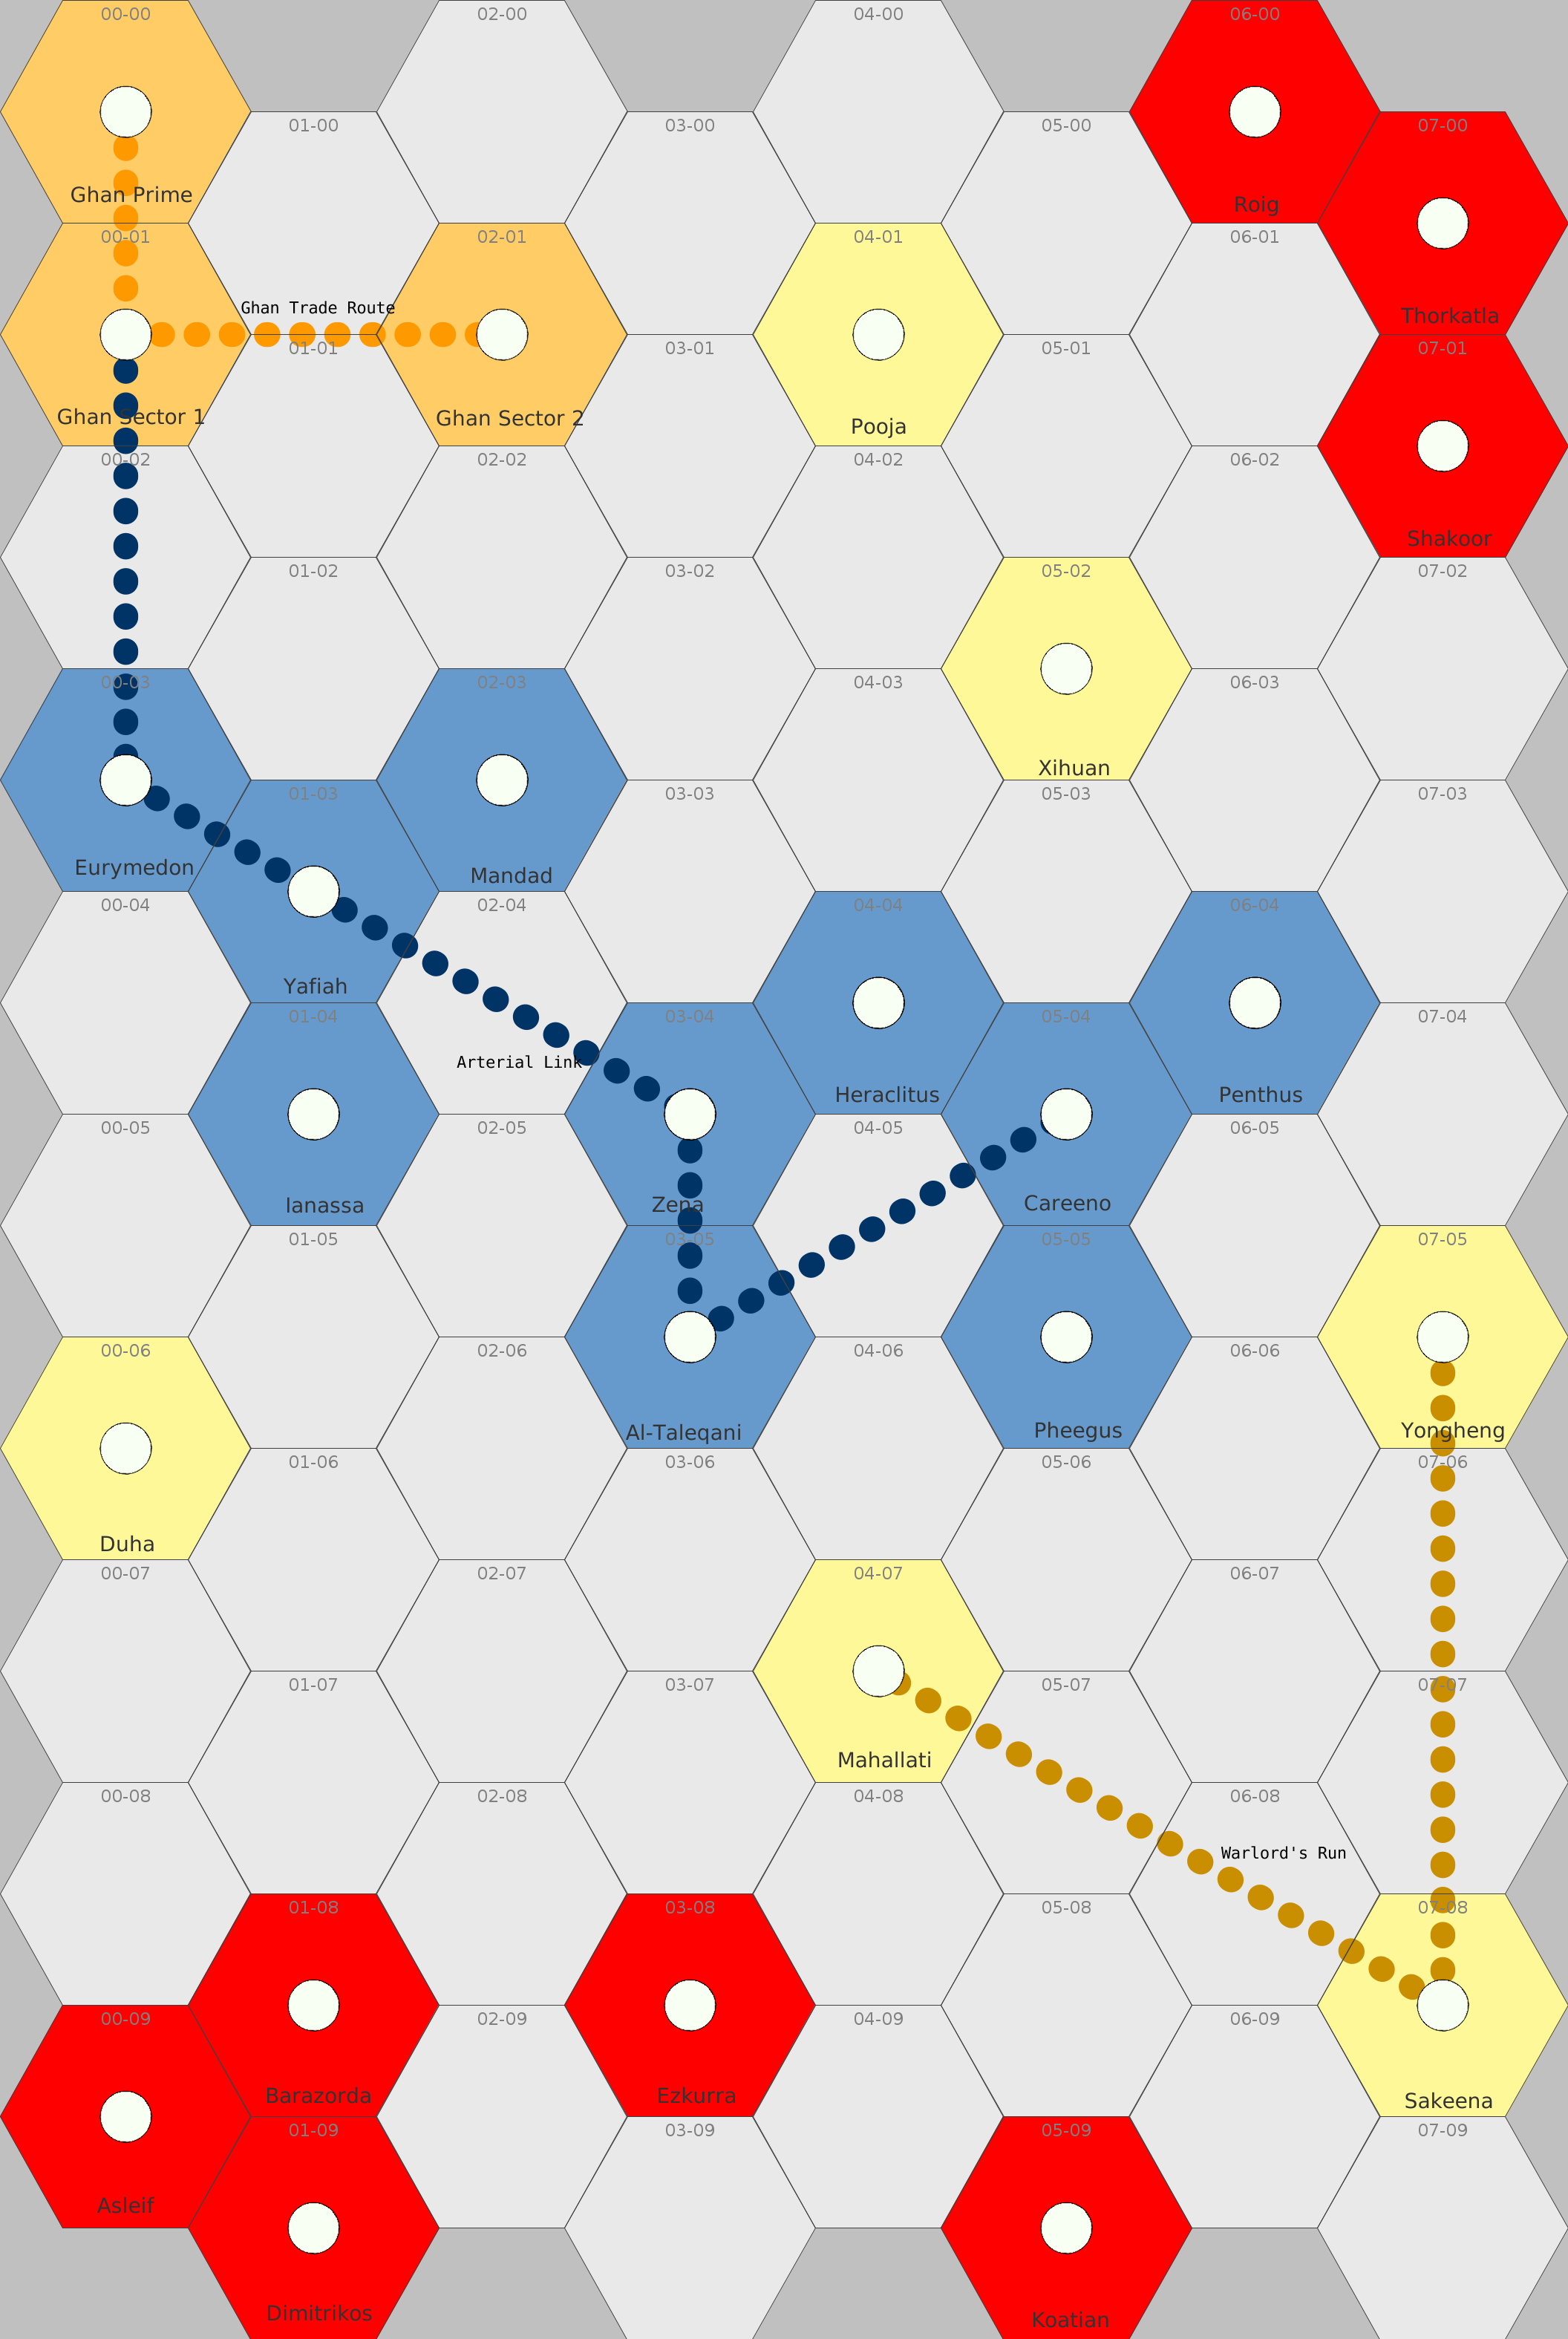
\includegraphics[height=220mm]{sectormap}
  \end{center}
  
  \newpage
  
  \begin{multicols}{2}
  
  \subsection{Star Systems}
  
  Sector Shangra Omega consists of 10 \textit{Core} systems (blue), 6 \textit{Independent} systems (yellow), 3 \textit{Ghan} systems (orange) and possibly up to 8 \textit{Lost} systems (red). The sectors that surround Shangra Omega are largely unexplored, and ancient star charts are severely out of date. The sector map used by navigators today are the result of intrepid explorers braving the Black and re-charting the stars.
  
  Core systems are those that make up the \textbf{United Systems}, a loose federation of star systems that share a common legal framework and similar military structures. Planets and Star Systems are allowed to govern themselves, but are subject to Universal Decrees voted upon by the United Systems Council. Each star system sends 10 Delegates to the Council (regardless of the number of planets, colonies, space stations, or other habitation in that system), and Delegates do not necessarily need to be democratically appointed.
  
  Independent systems are those that choose to remain seperate from the United Systems. Some chose not to join because they feel that the strict 10 Delegates per system would unfairly discriminate their large populations. Others because the Decrees do not align with their local laws and customs. And some wish to remain black market havens. Whatever the reason, Independent systems are considered the "Wild West" of the Black.
  
  Ghan systems are, quite simply, the home systems for the Ghantak. Ghan Prime has the homeworld of Ghan, and the Ghantak were able to colonise (at least) two other star systems before the Surge. These systems have all managed to survive the Surge and re-establish contact with each other, but choose to remain seperate from the United Systems. They are led by an Empress who resides in Ghan Prime, but each planet is governed by a Hive Queen that has the freedom to do as she pleases.
 
  Lost systems are those that are speculated to still exist, but no formal communication or expedition exist to explore them fully. Travel to the Lost systems are fraught with danger, as many do not return.
  
  \columnbreak
  
  \begin{standardtable}{\linewidth}{bsb}
    \textbf{Name} & \textbf{Sector} & \textbf{Type}\\
    Al-Taleqani & 03-05 & Core\\
    Asleif & 00-09 & Lost\\
    Barazorda & 01-08 & Lost\\
    Careeno & 05-04 & Core\\
    Dimitrikos & 01-09 & Lost\\
    Duha & 00-06 & Independent\\
    Eurymedon & 00-03 & Core\\
    Ezkurra & 03-00 & Lost\\
    Ghan Prime & 00-00 & Ghan\\
    Ghan Sector 1 & 00-01 & Ghan\\
    Ghan Sector 2 & 02-01 & Ghan\\
    Heraclitus & 04-04 & Core\\
    Ianassa & 01-04 & Core\\
    Koatian & 05-09 & Lost\\
    Mahallati & 04-07 & Independent\\
    Mandad & 02-03 & Core\\
    Penthus & 06-04 & Core\\
    Pheegus & 05-05 & Core\\
    Pooja & 04-01 & Independent\\
    Roig & 06-00 & Lost\\
    Sakeena & 07-08 & Independent\\
    Shakoor & 07-01 & Lost\\
    Thorkatia & 07-00 & Lost\\
    Xihuan & 05-02 & Independent\\
    Yafiah & 01-03 & Core\\
    Yongheng & 07-05 & Independent\\
  \end{standardtable}
  
  \subsection{Tech-Levels}
  
  \begin{standardtable}{\linewidth}{ssb}
    \textbf{Level} & \textbf{Description} & \textbf{Example}\\
    0 & Primitive & Stone, human power\\
    1 & Basic & Metals, domestic animals, steam engine\\
    2 & Industrial & Fossil fuels, factories, simple machines\\
    3 & Electronic & Computers, satellites, 20th century era tech\\
    4 & Interstellar & IDD, energy weapons, cyberware \\
    5 & Advanced & Specialized knowledge in a technological field\\
    6 & Pre-Surge & Psionic tech, TDD, exotic tech\\
  \end{standardtable}
  
  \end{multicols}
  
  \newpage
  
  \subsection{Core Worlds}

  \begin{powertable}{ p{.10\textwidth} p{.10\textwidth} p{.05\textwidth} p{.10\textwidth} p{.05\textwidth} p{.05\textwidth} p{.10\textwidth} p{.25\textwidth} }
    \textbf{Name} & \textbf{Atmo.} & \textbf{Temp} & \textbf{Biosphere} & \textbf{Pop.} & \textbf{TL} & \textbf{Sector} & \textbf{Tags}\\
    Al-sahhah & Breath. & Vary & Compatible & 10B+ & 4 & Al-Taleqani & Trade Hub, Heavy Industry\\
    Androcles & Breath. & Temp. & None & 100K+ & 3 & Ianassa & Freak Geology, Quarantined\\
    Arantza & Thin & Warm & Compatible & 1M+ & 4 & Mandad & Restrictive Laws, Primitive Aliens\\
    Ballesteros & Thick & Temp. & Compatible & 10M+ & 4 & Pheegus & Rigid Culture, Seagoing cities\\
    Bergthora & Thin & Temp. & Hybrid & 1M+ & 5 & Penthus & Heavy Industry, Theocracy\\
    Mecisteus & Breath. & Temp. & Compatible & 1B+ & 4 & Yafiah & Banking, Diplomats, Local Tech\\
    Merlo & Breath. & Temp. & Incompat. & 1M+ & 3 & Mandad & Psionic School, Quarantined\\
    Olaria & Unbreath. & Temp. & Compatible & 1B+ & 5 & Eurymedon & Pre-Surge Cultists, Xenophiles\\
    Raghd & Breath. & Temp. & None & 10B+ & 5 & Carreno & Flying Cities, Major Spaceyard\\
  \end{powertable}
  
  \subsection{Independent Worlds}

  \begin{powertable}{ p{.10\textwidth} p{.10\textwidth} p{.05\textwidth} p{.10\textwidth} p{.05\textwidth} p{.05\textwidth} p{.10\textwidth} p{.25\textwidth} }
    \textbf{Name} & \textbf{Atmo.} & \textbf{Temp} & \textbf{Biosphere} & \textbf{Pop.} & \textbf{TL} & \textbf{Sector} & \textbf{Tags}\\
    Amir & Breathable & Temp. & Compatible & 1M+ & 4 & Duha & Oceanic World, Fear of Psionics\\
    Dirce & Breath. & Vary & Compatible & 100K+ & 4 & Pooja & Desert World, Civil War\\
    Garrastazu & Breath. & Temp. & Hybrid & 1M+ & 3 & Duha & Sectarians, Heavy Mining\\
    Sakeena & Thick & Temp. & Incompat. & 1B+ & 5 & Sakeena & Major Spaceyard, Police State\\
    Theano & Breathable & Frozen & Incompat. & 100K+ & 4 & Yongheng & Outpost, Hatred\\
    Vinata & Unbreath. & Warm & Compatible & 1M+ & 4 & Mahallati & Civil War, Bubble Cities\\
    Vargos & Thick & Temp. & None & 10B+ & 3 & Yongheng & Cold War, Warlords\\
  \end{powertable}
  
  \subsection{Lost Worlds}

  \begin{powertable}{ p{.10\textwidth} p{.10\textwidth} p{.05\textwidth} p{.10\textwidth} p{.05\textwidth} p{.05\textwidth} p{.10\textwidth} p{.25\textwidth} }
    \textbf{Name} & \textbf{Atmo.} & \textbf{Temp} & \textbf{Biosphere} & \textbf{Pop.} & \textbf{TL} & \textbf{Sector} & \textbf{Tags}\\
    Akriti & Thin & Temp. & Compatible & 10K+ & 2 & Koation & Zombies, Out of Contact\\
    Chloe & Breath. & Temp. & Compatible & 100K+ & 2 & Barazorda & Minimal Contact, Fear of Tech\\
    Echepolos & Breath. & Temp. & Microbial & 10K+ & 4 & Shakoor &  Radioactive, Tomb World\\
    Gyda & Breathable & Cold & Compatible & Failed & 3 & Ezkurra & Xenophobes, Pre-Surge Archive\\
    Maqsood & Breath. & Cold & Hybrid & 100K+ & 0 & Dimitrikos & Psionic Worship, Out of Contact\\
    Purva & Breath. & Frozen & Compatible & 100K+ & 3 & Dimitrikos & Feral, Pre-Surge Cultists\\
    Sagari & Breathable & Temp. & Compatible & 10K+ & 4 & Thorkatia & Hostile Space, Badlands World\\
  \end{powertable}
  
  \subsection{Ghan Worlds}

  \begin{powertable}{ p{.10\textwidth} p{.10\textwidth} p{.05\textwidth} p{.10\textwidth} p{.05\textwidth} p{.05\textwidth} p{.10\textwidth} p{.25\textwidth} }
    \textbf{Name} & \textbf{Atmo.} & \textbf{Temp} & \textbf{Biosphere} & \textbf{Pop.} & \textbf{TL} & \textbf{Sector} & \textbf{Tags}\\
    Ghan & Breath. & Temp. & Compatible & 10B+ & 5 & Ghan & Major Spaceyard, Local Speciality\\
  \end{powertable}
  
  \subsection{Corporations}

  \begin{powertable}{ p{.35\textwidth} p{.25\textwidth} p{.30\textwidth} }
    \textbf{Name} & \textbf{Business} & \textbf{Headquarters}\\
    Al-Astra Association & Heavy Weapons & Al-sahhah (Core)\\
    Anistonopoulos Clan & Banking & Mecisteus (Core)\\
    Cafu Pact & Weapons & Dirce (Ind.)\\
    Colonial Mining & Mining & Careeno (Core)\\
    Faraj Fishing & Fishing & Amir (Ind.)\\
    Ghan Systems & Xenotech & Ghan Prime (Ghan)\\
    Haen Multistellar & Art & Olaria (Core)\\
    Mavridou Cooperative & Aeronautics & Raghd (Core)\\
    Panstellar Zaibatsu & Construction & Ballesteros (core)\\
    Nopoulos Partnership & Fishing & Ballesteros (Core)\\
    Sakeena Shipyards & Shipyards & Sakeena (Ind.)\\
    Spiker Group & Pharma., Drugs & Vinata (Ind.)\\
    Tatum Farming Collective & Livestock & Arantza (Core)\\
    West Wind Outfit & Weapons & Vargos (Ind.)\\
  \end{powertable}
  
  \subsection{Politics}

  \begin{powertable}{ p{.20\textwidth} p{.10\textwidth} p{.15\textwidth} p{.10\textwidth} p{.10\textwidth} p{.20\textwidth} }
    \textbf{Name} & \textbf{Ruler} & \textbf{Economy} & \textbf{Migrants} & \textbf{Homeworld} & \textbf{Issues}\\
    Buffalo Party & Rural & Laissez-faire & Hybrid & Arantza & Tradition, Immigration\\
    Cerulean Guild & Urban & State industry & Hybrid & Mecisteus & Government reform, Industry\\
    Cobalt Consensus & Bourgeoisie & Socialist & Xenophilia & Careeno & Welfare, Poverty\\
  \end{powertable}
  
  \newpage

  % =================
  % Terminology
  % =================

  \section{Lingo}

  \begin{multicols}{2}

  \begin{itemize}

    \item \textbf{AGI}: Artificial General Intelligence or "\textit{strong AI}". An AI that has cognitive faculties comparable to a human or higher.

    \item \textbf{AI}: Artificial Intelligence. Generally used for "\textit{weak AI}", or specialised AI that do not encompass the full range human-level cognitive abilities.

    \item \textbf{AR}: Augmented Reality. Information that is overlaid onto your real-world senses. AR data is usually visual, but can also be audio, tactile, olfactory, kinesthetic (body awareness), emotional, and other senses.

    \item \textbf{Ay-Matak}: (\textit{plural: Ay-Matakian}) Alien race that has evolved from birds native to their planet. The species have an innate wanderlust, and are never happy staying in one place too long. They place high social value in the areas of art, pleasure and excitement. Their political system is based on oligarchic rule by influential elders.

    \item \textbf{Black}: Slang term for space.
    
    \item \textbf{Core system}: A system in the Shangra Omega system that is part of the United Systems.

    \item \textbf{Cortical Stack}: An implanted electronic data storage used for memory and personality backups. Located where the spine meets the skull. Commonly known as a "\textit{Stack}".

    \item \textbf{Cradle}: Slang term for Earth. Location is currently unknown.

    \item \textbf{Credit}: Standard interchangeable monetary unit accepted by most space-faring worlds. Issued as either electronic banking entries, or embedded onto physical electronic chips. Some primitive worlds use "notes" made of plastic or paper.

    \item \textbf{Cyberware}: Generic term for the neural interface technology that melds metal and flesh into a coherent whole. This technology enables AR, Cortical Stacks, Ghosts in their Shells, and Sim-Sense. Commonly known as a "\textit{Warez}".

    \item \textbf{ECM}: Electronic Counter Measures. A suit of electronic tools designed to target and cripple enemy sensors to make you almost impossible to track and hit. Commonly known as a "\textit{E-War}" or "\textit{iWar}".

    \item \textbf{FTL}: Faster-Than-Light.

    \item \textbf{Ghantak}: (\textit{plural: Ghantakian}) Alien species that have evolved from beetle-like insects native to their planet. The species place a high value on honour and tradition, with a singular Queen ruling over the entire species. Personal sacrifice for the sake of upholding Ghantakian values earns you glory and esteem. The race favours traditional solutions to problems, and individuals are uncomfortable when forced to exercise their own judgement.
    
    \item \textbf{Ghan system}: The three star systems that include the native home of the Ghantak.

    \item \textbf{Ghoa}: (\textit{plural: Ghoan}) Alien species that have evolved from an unusual mammal-reptile hybrid native to their planet. The species are typically tribal, putting their tribe ahead of all other social groups (including the species as a whole). Their chief mode of expression is anger, and the Ghoa are prone to acts of wanton violence. Disputes are traditionally resolved through force (rarely to the death). Some Ghoa actively embrace the honour and glory of death in battle. Their political system is based entirely upon the tribe that the Ghoa is a part of.

    \item \textbf{Ghost}: Slang term used for a digitised persona. Some individuals have used Cortical Stacks to make a digital copy of themselves. These copies exist on digital hardware or in artifical bodies known as Shells. There is debate on whether these copies are really "people" or just another AGI.

    \item \textbf{IDD}: Intra-Dimensional Drive. Spaceship engine used to achieve FTL speeds based on TDD technology. To guard against another Surge-like event, IDD only manipulates Space-Time within a precisely defined spectrum. TDD does not have this limitation, and therefore TDD technology is vastly superior in performance and achievable FTL speeds.
    
    \item \textbf{Independent system}: A star system that chooses, for various reasons, to remain seperate from the United Systems.

    \item \textbf{Jump Portal}: Large gateways that used TDD technology to allow large cargo ships to travel at FTL speeds. All known portals are currently defective and inoperable.
    
    \item \textbf{Lost system}: A star system that is rumoured to still exist. Travellers tell of it's existance, but no formal expedition has been commissioned to verify the tails.

    \item \textbf{Muse}: Slang for personal AI helper programs.

    \item \textbf{Psionic}: An individual adversely affected by trans-dimensional energy. Some have been granted the ability to manipulate Space-Time, while others become malformed and driven mad. Also known as psychics, paranorms, and jsingshen.

    \item \textbf{Propulsion Thruster}: Conventional spacecraft engine that propels energy away from the spacecraft to create thrust. Used for interplanetary travel within a star system.

    \item \textbf{Reclaimers}: Euphemistic slang for scavengers. These individuals search and scour the Black for salvageable ruins.
    
    \item \textbf{Shangra Omega}: The name of the sector of the Black this setting takes place in. Nicknames includes "\textit{Shangra}", "\textit{Shomega}", and "\textit{Shang-o}".

    \item \textbf{Shell}: Slang term for an artificial body. These bodies can either be synthetic or biological. There is debate on whether these Shells are really "people" or just another Bot.

    \item \textbf{Sim-sense}: Experiencing someone else's sensory input (in real-time or recorded).

    \item \textbf{Space-Time}: The concepts of time and three-dimensional space fused in a four-dimensional continuum.

    \item \textbf{Splicer}: Slang for an individual that has undergone extensive genetic modification and transformation.

    \item \textbf{Surge}: A mysterious event that overloaded all technology that utilised trans-dimensional energy.

    \item \textbf{TDD}: Trans-Dimensional Drive. Heavy utilised technology that bends Space-Time to achieve FTL travel. A side effect is the creation of psionics.

    \item \textbf{Tech-Level}: Standard technology classification for worlds. There are seven tech-levels, ranging from 0 (stone-age) to 6 (advanced technology exceeding anything from pre-Surge civilisation)

    \item \textbf{Trans-dimensional energy}: A form of energy that is the by-product of manipulating the multiple dimensions of Space-Time by collapsing and bending it. Not much is known about this energy despite it's importance to IDD and TDD technology.
    
    \item \textbf{United Systems}: A loose alliance of star systems that share a common legal and military framework.

    \item \textbf{Uplifted}: Animals that are biologically and geneticatlly engineered to have higher intelligence and sentience.

    \item \textbf{Xenomorph}: Alien life form. Also "\textit{xeno}", and includes the Ay-Matak, Ghantak, Ghoa, Kaj and Pluvma.

  \end{itemize}

  \end{multicols}

\end{document}
